\documentclass[twocolumn]{svjour3} 

\usepackage[square,sort,comma,numbers]{natbib}
\usepackage{graphicx}
\usepackage{amssymb,amstext}
\usepackage{url}

\journalname{Journal on Multimodal User Interfaces}

\begin{document}

\title{A Computational Model for the Emergence of Turn-Taking Behaviors in User-Agent Interactions}

\author{Mathieu J\'egou  \and
        Pierre Chevaillier
}

\institute{M. J\'egou \at
              B-Com, France \\
              \email{mathieu.jegou@gmail.com}           %  \\
           \and
           P. Chevaillier \at
              Lab-STICC, ENIB, F-29280 Plouzan\'e, France
}

\date{Received: date / Accepted: date}

\maketitle 

\begin{abstract}
We propose a computational model that endows conversational agents with the capability to coordinate their speaking turns in the context of mixed-initiative dialogs.
In human conversations, participants are continuously adjusting their verbal and non-verbal productions to adapt their behavior for ensuring  effective coordination. Turn-taking management is the process through which agents decide on whether to continue speaking (or listening). In our model, the decision making is a continuous process based on the intrinsic current goal of the agent with respect to turn-taking, namely, its motivation to keep its current role (speaker or listener) or to switch to the opposite role, and on its perception of the intentions of its partner. Concurrently, the agent is also producing signals indicating its willingness to maintain or leave its current role. Because all the participants in the interaction behave according to this principle, the actual coordination of speaking turns is an emergent property. This results from the continuous sensory-motor coupling of the interactants. Our model is based on two models from cognitive psychology: the drift-diffusion model and the theory of behavioral dynamics. After presenting simulations showing how our model makes the coordination emerge from the interactions, we propose a SAIBA-Compliant architecture, named BeAware, created to support the implementation of our model. Finally, using our model, we investigate how an agent's turn-taking strategy may impact the user's experience and the effectiveness of the coordination.

 
%Insert your abstract here. Include keywords, PACS and mathematical subject classification numbers as needed.
\keywords{Turn-taking \and User-Agent interaction \and Embodied conversational agent \and Prosody}
% \PACS{PACS code1 \and PACS code2 \and more}
% \subclass{MSC code1 \and MSC code2 \and more}
\end{abstract}

\section{Introduction}
\label{sec:intro}

According to Cassell et al. \cite{cassell_embodiment_1999}, embodied conversational agents are graphical entities that are able to interact naturally with users by producing and interpreting natural spoken language, co-verbal and non-verbal signals such as prosody, gestures, facial expressions, and gaze. 
To ensure natural interactions with the user, embodied conversational agents should be able to manage conversational functions such as turn-taking \citep{cassell_embodiment_1999}. Turn-taking refers to the ability of conversants to alternate speaking turns, such as only one participant speaks at a time, which is the most common \citep{sacks_simplest_1974}. Turn-taking encompasses two major abilities: the ability to seamlessly take turns by correctly interpreting the signals produced by the participants just before the end of the turn and the ability to address conflicting situations whereby both participants attempt to take the turn simultaneously \citep{thorisson_natural_2002}. 

Several authors have contributed to endowing conversational agents with natural turn-taking behaviors \citep{thorisson_natural_2002,raux_optimizing_2012,jonsdottir_distributed_2013}. However, user-agent turn-taking remains non-natural, far from what can be observed in human conversations. Indeed, the agent's decisions toward turn-taking are often controlled by simple rules: never speak at the same time the user is speaking; when the user interrupts you, stop speaking to let the user speak; and take the turn as soon as possible after the end of the user's turn \citep{ter_maat_how_2010}. Real conversations are more complex: short speech overlaps are not very rare, and conflictual situations, where both participants want to have the floor simultaneously, are also common. Moreover, the durations of silence between two turns are highly variable. This large variety of situations originates from different conversational factors, such as the interpersonal attitudes of the participants, their personality traits \citep{ter_maat_how_2010} and the type of verbal contributions of the agents \citep{cafaro_effects_2016}. However,  few turn-taking models have considered these factors \citep{lessmann_towards_2004,ravenet_conversational_2015}.
Moreover, current models of turn-taking follow the perceive-decide-act paradigm: agents make punctual decisions about how to behave regarding turn-taking after having gathered sufficient information about the user's behavior. This results in long response latencies of the agent and poor abilities to address conflictual situations, far from the smoothness characterizing human interactions. We argue that the ability of an agent to exhibit natural turn-taking behaviors in this context requires that the agent be able to perceive, decide and act continuously and concurrently.  

In this article, we propose a computational model that makes a conversational agent able to coordinate its speaking turns with the user in the context of mixed-initiative dialogs while allowing the agent to vary its turn-taking behavior to better reproduce the complexity of situations observed in human interactions. 
Our proposal is grounded in the behavioral dynamic theory promoted by Warren \cite{warren_dynamics_2006}, which leads us to assume that the exchanges of turns are not under the control of a single participant but rather are the result of their sensory-motor coupling. Specifically, both participants are continuously adapting their production of verbal and non-verbal signals according to the current behavior of their partner. Therefore, the coordination of the speaking turns is an emergent property of the interaction in the sense of \cite{warren_dynamics_2006}. 

In the remainder of this article, we first present existing work on human and user-agent turn-taking and justify our approach. 
We then present our theoretical model and describe its properties based on simulated agent-agent interactions. These simulations highlight the ability of the model to qualitatively reproduce situations observed during human conversations. 
We also show that the model allows the agent to adapt to its environmental setting and, more importantly, that this adaptability is not due to a process explicitly formulated in our model but rather is a property that emerges from the interaction. 
Next, we present BeAware, the computational architecture that we propose to implement the model in the context of real-time user-agent dialogs, making our turn-taking model work together with components dedicated to the interpretation and generation of verbal utterances. The solution, which is based on ASAP \cite{kopp_architecture_2014} and implements some principles of Ymir \cite{thorisson_mind_1999}, supports the implementation of both event-driven rule-based models and continuous emergent models. 
Finally, we conclude the article by analyzing the real-time interactions between an agent controlled by our model and a user. 
 This evaluation is aimed at analyzing the ability of both our agent and the user to coordinate their turns. 

\section{Background and motivations}
\label{backgd}

\subsection{How do human participants manage their turns?}
\label{social_psychology}

One of the most noticeable properties of turn-taking in human conversation is that participants often take turns smoothly \citep{heldner_pauses_2010}, with the duration of silence between two turns lasting a few hundreds of milliseconds. 
It should be noticed that this principle varies across cultures, languages and types of conversation \citep{oconnell_turntaking_2008,stivers_universals_2009}.
However, the principle applies to French conversations \citep{mondada_multimodal_2007}, which represent the type of conversation to which our model applies.
The smoothness of conversations remains an open issue to researchers interested in the study of human conversations, and several models have been elaborated upon. 
 
Sacks et al. \citep{sacks_simplest_1974} proposed the most widely known model explaining how participants coordinate their spea\-king turns.
They consider that a set of rules ensures the coordination of turns, enabling the smooth transitions observed during conversations.
More precisely, speaking turns are composed of Turn Constructional Units (TCU): groups of words or several sentences that the listener, the participant that does not possess the turn (in contrast, the speaker is the owner of a turn), perceives and uses to precisely identify moments that are appropriate to initiate a turn transition, moments known as Transition Relevant Places (TRPs).

For Sacks et al. \citep{sacks_simplest_1974}, at these TRPs, any deviation from this set of rules is considered as a violation of the turn-taking system, and a repair mechanism should be applied to address this situation.
Such violations of the turn-taking mechanism characterize listeners that attempt to take the turn outside a TRP, leading to competitive overlaps \citep{schegloff_overlapping_2000}.
This first approach is based on the assumption that listeners are able to predict precisely the current speaker's end of turn based on the multimodal behavior of the latter \citep{de_ruiter_projecting_2006,french_turncompetitive_1983,ford_interactional_1996,mondada_multimodal_2007}. 

While being the most widely used and cited approach, other approaches have challenged the model developed by Sacks et al. \citep{sacks_simplest_1974}.
As an alternative to the prediction approach, the Signal Reaction Approach, presented by Duncan \citep{duncan_signals_1972}, does not follow this assumption of prediction made by Sacks et al. nor does it assume the existence of a rule system controlling TRPs. 
The authors following this approach consider that the coordination of speaking turns is mainly the result of a negotiation process whereby both the speaker and the listener actively act toward taking the turn.

More precisely, according to \citep{bunt_dimensions_2006}, participants can perform the following actions to ensure the coordination of speaking turns: 
\begin{itemize}
\item take the turn: the current listener seizes a turn that is available,
\item grab the turn or interrupt: the current listener attempts to seize a turn that is not available,
\item keep the turn: the current speaker signifies its willingness to continue speaking in the case of a pause or in the case of a listener attempting to take the turn,
\item release the turn: the current speaker makes the turn available to the current listener.
\end{itemize}

According to Duncan, to coordinate, participants exchange verbal and non-verbal signals that inform the different actions that they undertake to facilitate the coordination of speaking turns. 
Several turn-releasing, turn-taking, turn-grabbing and turn-keeping signals have been identified since the seminal article from Duncan \citep{duncan_signals_1972}. These signals encompass, for instance, variations in prosody \citep{duncan_signals_1972,gravano_turn-taking_2011,hjalmarsson_additive_2011}, gesture \citep{duncan_signals_1972,mondada_multimodal_2007}, gaze \citep{kendon_functions_1967,novick_coordinating_1996,oertel_gaze_2013} and vocal patterns 
such as fillers \citep{benus_pragmatic_2011} and inbreath \citep{torreira_breathing_2015}.  

Recent work in psychology has criticized the assumption of the two preceding approaches, claiming that turn-taking is an affair of ``rights'' and ``obligations''. O'Connell et al.\citep{oconnell_turn-taking_1990} argued that ``the ultimate criterion for success in conversation is not the smooth interchange of speaking turns [...] but the fulfillment of the purpose entertained by participants". According to their view, turn-taking does not exist per se as an independent procedure deliberately undertaken by the participants; rather, the way participants exchange turns is grounded in the situational and environmental context of the conversation.
Thus, several contextual factors, such as interpersonal attitudes \citep{ter_maat_how_2010}, the nature of the verbal contributions \citep{clark_using_1996,cafaro_effects_2016} or emotions \citep{goldberg_interrupting_1990}, influence the agent's turn-taking behavior. 

This means that creating an agent able to vary its own behavior related to turn-taking, such as choosing to interrupt the user if it has something important to say
or allowing a certain amount of silence before
taking the turn, would not degrade the interaction; in contrast,
if it is made coherently with the dialog context, this behavior would enrich the interaction. This view has been
supported by recent studies made by \citep{ter_maat_how_2010} and \citep{cafaro_effects_2016}, who measured
the effects of different turn-taking behaviors (referred to as ``strategies") on
the user's perception of the agent.
ter Maat et al.\citep{ter_maat_how_2010} showed that varying the response time of the agent following the end of a user's turn resulted in different impressions about the personality and attitude of the agent toward the user. They showed that an agent starting systematically a few hundred milliseconds before the end of the user's turn was perceived as more dominant and assertive, and in contrast, an agent taking a turn seconds after the end of the user's turn was perceived as less assertive and more submissive.  
Cafaro et al.\citep{cafaro_effects_2016} studied the effects of different interruption strategies (cooperative or disruptive) on the user's
perception about the engagement, interpersonal attitude
and involvement of agents. They found that the type of interruption (whether it is a slight overlap at the very end of the previous turn, an interruption made while the current speaker was pausing or while the current speaker was speaking), more than
the disruptive or cooperative strategy employed by the
agent, influenced the user's perception about the interpersonal
attitudes of the participants.
 
Previous studies have demonstrated the existence of turn-taking signals but have not observed the dynamics of such signals.
Some authors specifically studied the dynamics of turn-taking signals and showed that participants continuously adapted their turn-taking signals to the other participant, leading to the belief that a continuous sensorimotor coupling occurred (for a definition of sensorimotor coupling, see \citep{warren_dynamics_2006}).
For instance,  Levitan et al. \citep{levitan_entrainment_2015} observed some
alignment effects in the amount of silence before participants
take the turn, and they showed that the pitch level of
the next speaker at the beginning of the turn tended to
be similar to the prosody level of the previous speaker
at the end of his turn. 
Alignment effects have also been observed in respiratory patterns close to the current speaker's end of turn \citep{mcfarland_respiratory_2001}.
Finally, Wilson and Zimmerman \citep{wilson_structure_1986} for English conversations and Bailly et al. \citep{bailly_pauses_2012} for French ones observed that inter-turn transitions were not randomly distributed but rather were multiples of a unit of time. According to \citep{wilson_oscillator_2005}, this could be explained by an alignment in the cycle of the pronunciation of syllables between the current speaker and the next speaker.

\subsection{Computational models of turn-taking for embodied conversational agents}
\label{comp_modelling}

The main goal of computational models of turn-taking for user-agent interactions is to satisfy the strict sequencing of speaking turns between users and agents, mostly in
dyadic settings, by accurately detecting when the user has finished speaking while differentiating pauses from ends of turns. Accurately recognizing user's ends of turns
will decrease the involuntary overlaps of the agent linked to poor perceptions of a user's end of turn and will make the durations of silence between the user's end of turn and the agent's beginning of turn as short as those observed in human conversations \citep{balentine_debouncing_1997,ward_root_2005,raux_optimizing_2012,jonsdottir_distributed_2013}.

The simplest approaches use fixed temporal thresholds to determine whether a silence can be considered as the end of the user's turn or a pause. 
These approaches have been proven to be inefficient, therein decreasing the smoothness of interaction between the user and the agent \citep{ward_root_2005}. 
To overcome these limitations, some authors have used a mechanism of dynamic thresholding for the agent to adapt to the
situation and to the user \citep{bohus_decisions_2011,witt_modeling_2014}. To improve the accuracy of the recognition of the user’s actions, linked to turn taking (turn releasing, keeping, taking, and grabbing), authors following the Signal Reaction Approach \citep{duncan_signals_1972} have attempted to perceive different signals displayed by the user to inform his current behavior linked to turn-taking.   
This encompasses rule-based systems \citep{cassell_embodiment_1999,thorisson_natural_2002} and probabilistic
models that use either a decision theoretic approach \citep{bohus_decisions_2011,raux_optimizing_2012}, offline machine learning on transcriptions of human conversations \citep{schlangen_reaction_2006,huang_multimodal_2011} or real-time reinforcement learning \citep{jonsdottir_distributed_2013} to accurately detect the user's ends of turns while discriminating ends of turns from simple pauses made by the user. 

In contrast, very few models have adopted Sacks et al.'s view that ends of turns are primarily projected. \citep{de_vault_incremental_2011} created a model dedicated to the prediction of the meaning of a user's utterance that could be applied in real time to generate interruptions or to take the turn with virtually no gap or overlap.

A second issue, more related to barge-in management,
was addressed by Reidsma et al. \citep{reidsma_continuous_2011}, Selfridge et al.\citep{selfridge_continuously_2013}, Witt et al.\citep{witt_modeling_2014} and Paek et al. \citep{paek_continuous_2000}. This issue relates to observations that dialog systems often falsely detect user's utterances as barge-ins, whereas the latter is only providing feedback to the system by producing a vocal backchannel or is not speaking to the system. Several studies have thus explored how a spoken dialog system could reliably distinguish barge-in
attempts from cooperative feedback or speech not intended as toward the system. This was done by either analyzing the results of an incremental speech recognizer \citep{selfridge_continuously_2013}, estimating the probability of a user starting to speak at a moment during the interaction \citep{witt_modeling_2014} or using a classifier to use prosodic, temporal and verbal features to distinguish between user's competitive overlaps and listener responses \citep{reidsma_continuous_2011}. Finally, Paek et al. \citep{paek_continuous_2000} used gaze to infer whether a user's utterance is addressed to the system. 

Several authors have designed agents that produced turn-taking signals to clarify their intentions related to turn-taking. In multi-party conversations between users and virtual agents or robots, several approaches have demonstrated the effectiveness of controlling the agent's gaze behavior for selecting the future speaker \citep{mutlu_storytelling_2006,bohus_facilitating_2010,al_moubayed_regulating_2015}. In dyadic settings, \citep{skantze_turn-taking_2014} showed that an agent averting its gaze when pausing (but not releasing its turn) helped the user to identify the agent's turn-taking behavior.

The models presented above are essentially dedicated to the detection of the user's behavior. They aim at reducing moments of silence and overlaps, thus improving the quality of the interaction. 
They partly rely on the initial assumptions that interrupting or not taking a turn after the user's end of turn is a violation of the turn-taking system and could lead to a ``break down" in the conversation \citep{cutler_analysis_1986}. 
Thus, in user-agent interactions,  the agent is seen as having ``obligations" toward
taking a turn without providing excessive silence and not interrupting the user \citep{de_kok_multimodal_2009}.

In contrast, several authors have created computational models of turn-taking for user-agent and agent-agent interactions that varied the agent's turn-taking behavior by controlling 
different variables. 
Selfridge et al. \citep{selfridge_bidding_2009} created a model for a dyadic agent-agent setting, where the goals of the agents toward the turn (take, grab, release, keep the turn) were mostly driven by the importance of the utterance that they had to produce. To evaluate whether they will take the turn, the agents evaluated in parallel the importance of the utterance that they had or were producing and the turn-holding or turn-taking cues displayed by their partner to judge whether to take the turn or keep the turn. Le{\ss}mann et al. \citep{lessmann_towards_2004} and Thorisson et al. \citep{thorisson_multiparty_2010} both used similar concepts of ``intention to speak" \citep{lessmann_towards_2004} or ``urgency to speak" to drive the behaviors of their agents \citep{thorisson_multiparty_2010}. Ravenet et al. \citep{ravenet_conversational_2015} created a model wherein the participants varied their behavior related to turn-taking based on their interpersonal attitudes. To achieve a richer and more natural turn-taking behavior, these models take into account factors related to personality, interpersonal attitude, emotion and the content of the conversation in the control of the agent's behavior. 

\subsection{Positioning}

Accurately detecting the behavior of the user is a first step toward improving the coordination of speaking turns. More complex approaches allow the agent to vary its behavior by applying "turn-taking strategies" \citep{ter_maat_how_2010} to display attitudes of dominance or power toward the user \citep{ravenet_conversational_2015,cafaro_effects_2016}. 

These approaches share certain characteristics. Upon achieving a high degree of certainty about the partner's behavior, agents make punctual decisions about the current behavior to trigger (either taking, releasing, grabbing, or keeping the turn) and do not  revise their decision often.
In contrast, participants in human interactions continuously perceive and react to their partner's behavior \citep{clancy_co-constructed_2015}. Indeed, participants continuously adapt their signal production to the behavior of their partner, and their final behaviors (the speaker either stops or continues to speak and the listener either takes the turn or does not) cannot be planned in advance. For example, the current speaker attempting to keep a turn can display signals indicating to the current listener that he wants to keep the turn, therein deciding to raise its voice, increase his speech rate, or constantly repeat the last syllable, as shown by Schegloff \citep{schegloff_overlapping_2000}. These behaviors are continuously dependent of what the listener is doing: if the listener insists on attempting to take the turn, the current speaker can choose to increasingly insist on keeping the turn (for instance,  increasing the volume of its voice to prevent the current listener from taking a turn), and then, as the overlap is continuing, the speaker can finally interrupt himself to let the listener take the turn \citep{schegloff_overlapping_2000}.  
A similar observation can be made for a listener engaged in a conflict for grabbing the turn: he can amplify his turn-grabbing signals, ultimately giving up on its turn-grabbing attempt.
The behaviors of the participants are then highly dynamic, continuously evolving throughout the interaction, and are directly dependent on the signals produced by their partner. In this sense, turn-taking behaviors cannot be entirely determined by the agent and are rather  a result of both an initial goal (taking, yielding, or keeping the turn) and a continuous adaptation to the partner's actions. Existing models lack an explanation of how participants can smoothly coordinate their turns by continuously adapting to their partner's signals.  
 
Moreover, as observed by \cite{thorisson_natural_2002}, participants coordinating their turns are under temporal constraints; they act regardless of whether they are completely certain about the intentions of their partners toward turn-taking, that is, whether their partners are attempting to change role (from listener to speaker and vice versa). This can be the case, for instance, for a listener waiting for the end of the speaker's turn to take the turn, even if he is not completely certain about the nature of the speaker's silence (whether he is only pausing or if he has ended his turn) as the silence continues, he will certainly finish by acting toward taking a turn.
 	
 These two characteristics, continuous adaptation to the partner's behavior and action under uncertainty, are not new in the field of embodied conversational agents. Recent works have emphasized the need for agents  to be able to incrementally perceive the user's behavior and to react to it before the user's behavior ceases. These types of models have been applied to the management of the dialog between users and agents \cite{skantze_towards_2010} or backchannel eliciting behaviors \cite{buschmeier_when_2014}. For developing agents that are able to incrementally process and react to the user's behavior, \cite{kopp_architecture_2014} proposed the ASAP architecture, therein extending the SAIBA architecture by adding the ability to continuously perceive the behavior of the user and to adapt the ongoing behavior of the agent accordingly. 
 
 Nevertheless, to our best knowledge, no model has applied this principle of continuous perception and action to turn-taking; our aim was to create such a model. 

\subsection{Our Model}

We propose a generative model of turn-taking motivated  by both cognitive psychology models and studies
that measured alignment or synchrony effects without postulating the nature of the cognitive processes
behind these phenomena. This model is based on cognitive psychology theories that describe the
processes behind the continuous sensorimotor coupling between participants during their interaction and that
drive the agent's behavior.

Several authors have taken the perspective of a dynamic approach of cognition, as conceptualized by Kelso \cite{kelso_coordination_2009} and Warren \citep{warren_dynamics_2006}, to model different coordination phenomena such as 
the coordination of oscillating members \citep{haken_theoretical_1985}, 
the locomotion of pedestrians attempting to avoid each other \citep{rio_follow_2014}, and, 
for human conversations, the coordination of postures \citep{fowler_language_2008}.
\citep{rio_follow_2014} used the behavioral dynamics theory conceptualized by \citep{warren_dynamics_2006} in their computational model of the coordinated motions of pedestrians. The behavioral dynamics framework formulates the control of action by a set of dynamical systems, taking the form of differential equations with control variables that vary in real time based on variations in the information provided by the environment.
By precisely defining behavior as a set of dynamical systems, the framework provides strong principles for the
implementation of computational models derived from the theoretical principles. 
We then used the behavioral dynamics framework to formulate our model. 
Nevertheless, behavior dynamics does not explain how participants control 
their actions while being themselves uncertain about their partner's behavior. 

While perceiving their partner's current behavior, the agents are involved in a perceptual decision-making task based on the perception of the variations in the signals produced by their partners. Being the current speaker, the agent has to discriminate between two alternatives: is the current listener about to take the turn or not? Symmetrically, being the current listener, the agent has to determine whether the speaker is about to yield or keep the turn. The agent's decision is based on the variation in the signals produced by the other agents during the interaction that the agent can more or less likely perceive.

These conditions of uncertainty and dynamic choice between two alternatives follow the Two Alternative Forced Choice task paradigm (TAFC). This paradigm is extensively used in cognitive psychology to account for
the dynamics of the perceptual decision making of human agents, which have to discriminate the nature of the
stimuli that they are experiencing to make a decision \citep{bogacz_physics_2006}. Although several models of two alternative forced choice tasks have been created (see \citep{bogacz_physics_2006} for a review), one of the most widely used and simplest models is the Drift Diffusion Model (DDM) developed by Ratcliff \citep{ratcliff_theory_1978}. 
We chose to use this model to control how our agent perceives the behavior of its partners based on the multimodal signals displayed by the latter. 

 We postulate that a principle of perception and action in parallel applies to the coordination
of turns in human conversations. We assume that the agents are continuously perceiving the multimodal signals
produced by their partners and that they modulate in parallel their own actions (verbal and non-verbal
productions) according to the degree of certainty that they have toward the nature of the behavior of their partners.
In turn, by modulating their own productions, the agents can  produce signals early that are perceived by
their partners and that can push the latter to modulate their own signals according to their current goal
(taking or yielding the turn). This strong sensorimotor coupling may provoke the beginning of a turn or the end
of a turn earlier than if the agent were to simply passively interpret the signals of its partner without acting in parallel. 
The result is a tight coordination between the agents that could partly explain the different turn-taking patterns observed in human interactions. 

\section{Theoretical model}
\label{mod_pres}

\subsection{Overall architecture}

Concerning turn-taking management, depending of their current role in the conversation, the goals of the agents are as follows: being the current speaker, the agent's goals are to give the turn or to keep it; being the current listener, the agent's goals are to take the turn or to continue listening. Regardless of their current role (speaker or listener), the agents actively, indeed pro-actively, produce verbal and non-verbal signals according to their current goal. 
The signals that they produce also drive their behavior. For instance, in a given context, the current listener will start to speak if it has something to say and observes a variation in the signals produced by the current speaker indicating that it is about to end its turn. 
Thus, at any moment in time, and maybe at the same time, the agents have to decide whether they want to change their role (transitioning from speaker to listener or vice versa). However, the agents will not directly perform the corresponding communicative actions because they also consider the behaviors of the other agents. 
Finally, the time at which the turn will actually change results from the complex interplay of the individual behaviors of each agent. Moreover, the individual behaviors are controlled by two cognitive processes: the first process controls the agent's own motivation to change its role, and the second process controls the production of the communicative signals. 
Figure \ref{fig:mot} presents the two levels of dynamics involved in the control of the agent's behavior.

\begin{figure}
  \centering
  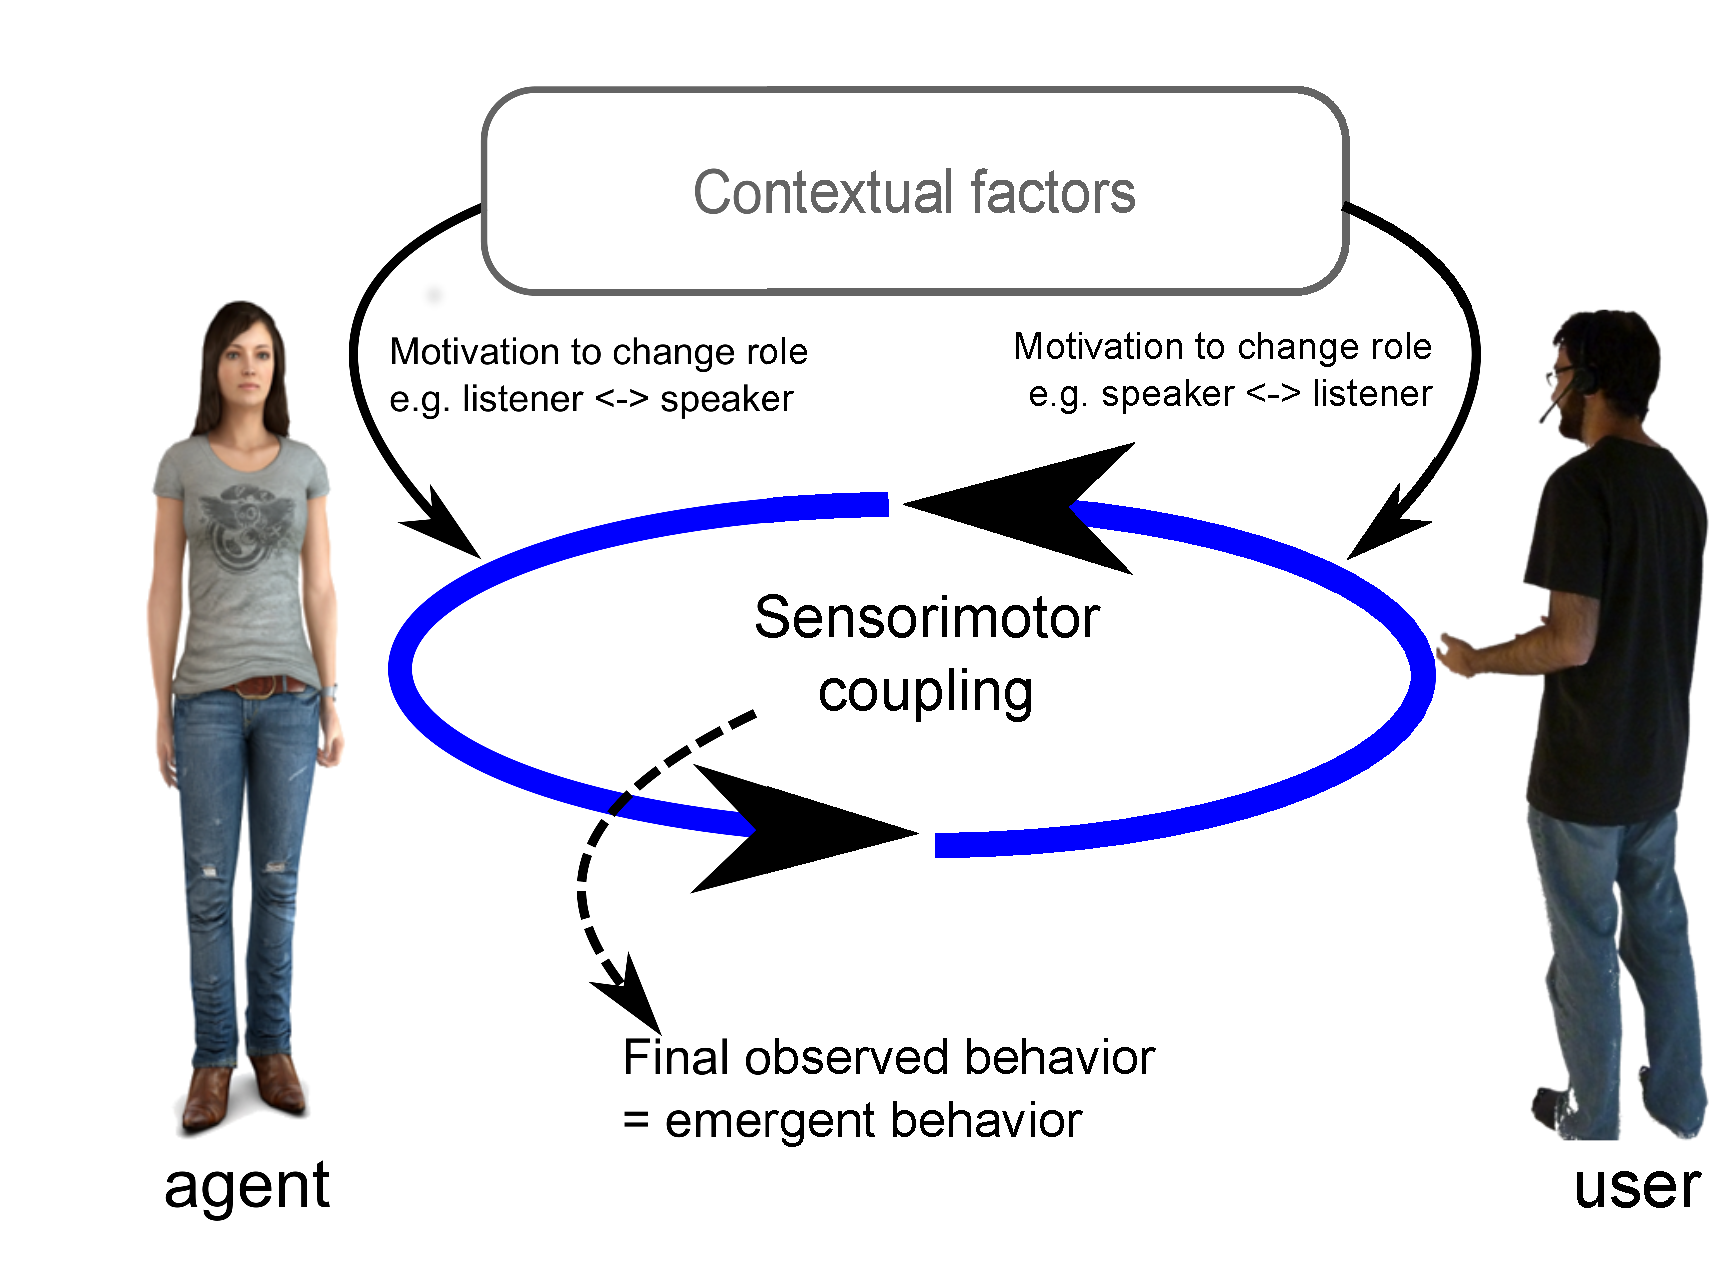
\includegraphics[width=\linewidth]{figure/schema_motivation.eps}

  \caption{The two levels of dynamics involved in turn-taking management. 
    Top level: the contextual factors, similar to the verbal productions, and the interpersonal attitudes vary the motivation each agent has in the current situation to change its role (being the speaker or the listener). 
Bottom level: the coordination process itself, partly driven by the agent's motivation and partly resulting from the sensorimotor coupling between the two participants. 
The observed behavior of the agents is an emergent property resulting from the interplay of the agents' behaviors.}
  \label{fig:mot}
\end{figure}

The first level at the top of the figure represents the contextual factors that impact how the agents attempt to take, release or maintain the turn. These contextual factors are numerous. Examples of these variables are the nature of the verbal contribution, especially the importance that the contribution has toward the progression of the dialog \citep{selfridge_bidding_2009}; its competitive or cooperative nature \citep{cafaro_effects_2016}; and the agent's attitude toward its partner \citep{ter_maat_how_2010} or the agent's emotions \citep{ter_maat_turn_2009}.

These factors influence, or modulate, the ``motivation'' of the agent to claim the turn when it is the current listener or to release the turn when it is the current speaker. 
In other words, these factors define the relative strength of the goals of each agent, namely, changing its role (speaker or listener) or continue keeping it. It is worth noticing that this motivation continuously varies during the interaction. 
What we call ``motivation" here is similar to what other authors have called ``urge to speak" \citep{thorisson_multiparty_2010} or ``intentions"  to speak \citep{lessmann_towards_2004} in the sense that it represents a variable that modulates the strength with which the agent will attempt to take or release the turn. We chose to call it ``motivation'' to remain as neutral as possible toward the contextual factors that could modulate this variable, as for example taking the turn early is not always related to an urgency to say something nor is it always related to explicit communicative intentions because a participant's emotions and attitudes can also impact the agent's behavior. 

In the  model, this motivation is a variable that continuously varies between $-1$ and $1$. 
$-1$ means that the agent has a strong motivation to keep its current role (listening or speaking), while $1$ means that the agent has a strong motivation to adopt the opposite role. 
The closer the value of the motivation is to $0$, the weaker the desire of the participant to change its role or to keeping it. 

The value of the motivation influences, but does not solely determine, the final behavior of the agent in terms of taking, yielding or keeping the turn. The motivation variable represents the goal of the agent toward turn-taking, but the final behavior of the agent is an emergent property of the interaction between the agent and its partner. 
This principle results from the second loop of the interaction in Figure \ref{fig:mot}. 
In this loop, the agent begins to vary its own signals regarding turn-taking (for example, decreasing loudness or pitch or gazing toward the user) based on its own goal as conveyed by the motivation variable. Nevertheless, the agent is coupled to its partner, and the signal production of its interlocutor directly influences how it will vary its own signals.
Conversely, the variation in its own actions will influence the behavior of its partner. 
As a result, the final behavior of the agent is an emergent property of the interaction between the participants.
This results from the complex interplay between the motivation of the participant and the cues given by its interlocutor.

\subsection{Scope of the modeling}

The objective of this study was the modeling of the continuous sensorimotor coupling between the participants. In this context, the motivation of the agent acts as a control parameter of the dynamics of this coupling. Thus, the law of control of this motivation is beyond  the scope of this work.
Moreover, our aim here is not to define the law of control for the production of the verbal and non-verbal signals, as observed in human conversations, but rather to model the general dynamics of the behavior and thus to capture how these various signals shape the agent's behavior. For the sake of generality, in the presentation of the theoretical model, we consider abstract values of these signals, and their variations are simplified on purpose, compared to what can be observed in human conversations.
For instance, the different prosodic features are treated as continuous variables, whereas in human conversations, their dynamics are linked to the phonemes produced by the participants. More precisely, the model accounts for a global evolution of the prosodic signals linked to the coordination of turns.
The same principle is followed for other signals mentioned in this article such as gestures and gaze directions. 
Another reason for this abstraction is to make the  theoretical model independent of the actual sensors and actuators that could be used for real-time interactions between the agent and the user. 
We will see in Section \ref{impl} the capacity of our implementation to adapt to a real interactive setup, and we will explain in greater detail how we used our theoretical values to modulate the prosody of the text-to-speech system.

\subsection{Components of the theoretical model}

We will now introduce in detail our theoretical model, which is divided into two components, as shown in Figure \ref{fig:mod-comp}: one component that is in charge of the continuous perception of the user's behavior and one component that controls the production of the different communicative signals. 

\begin{figure}
  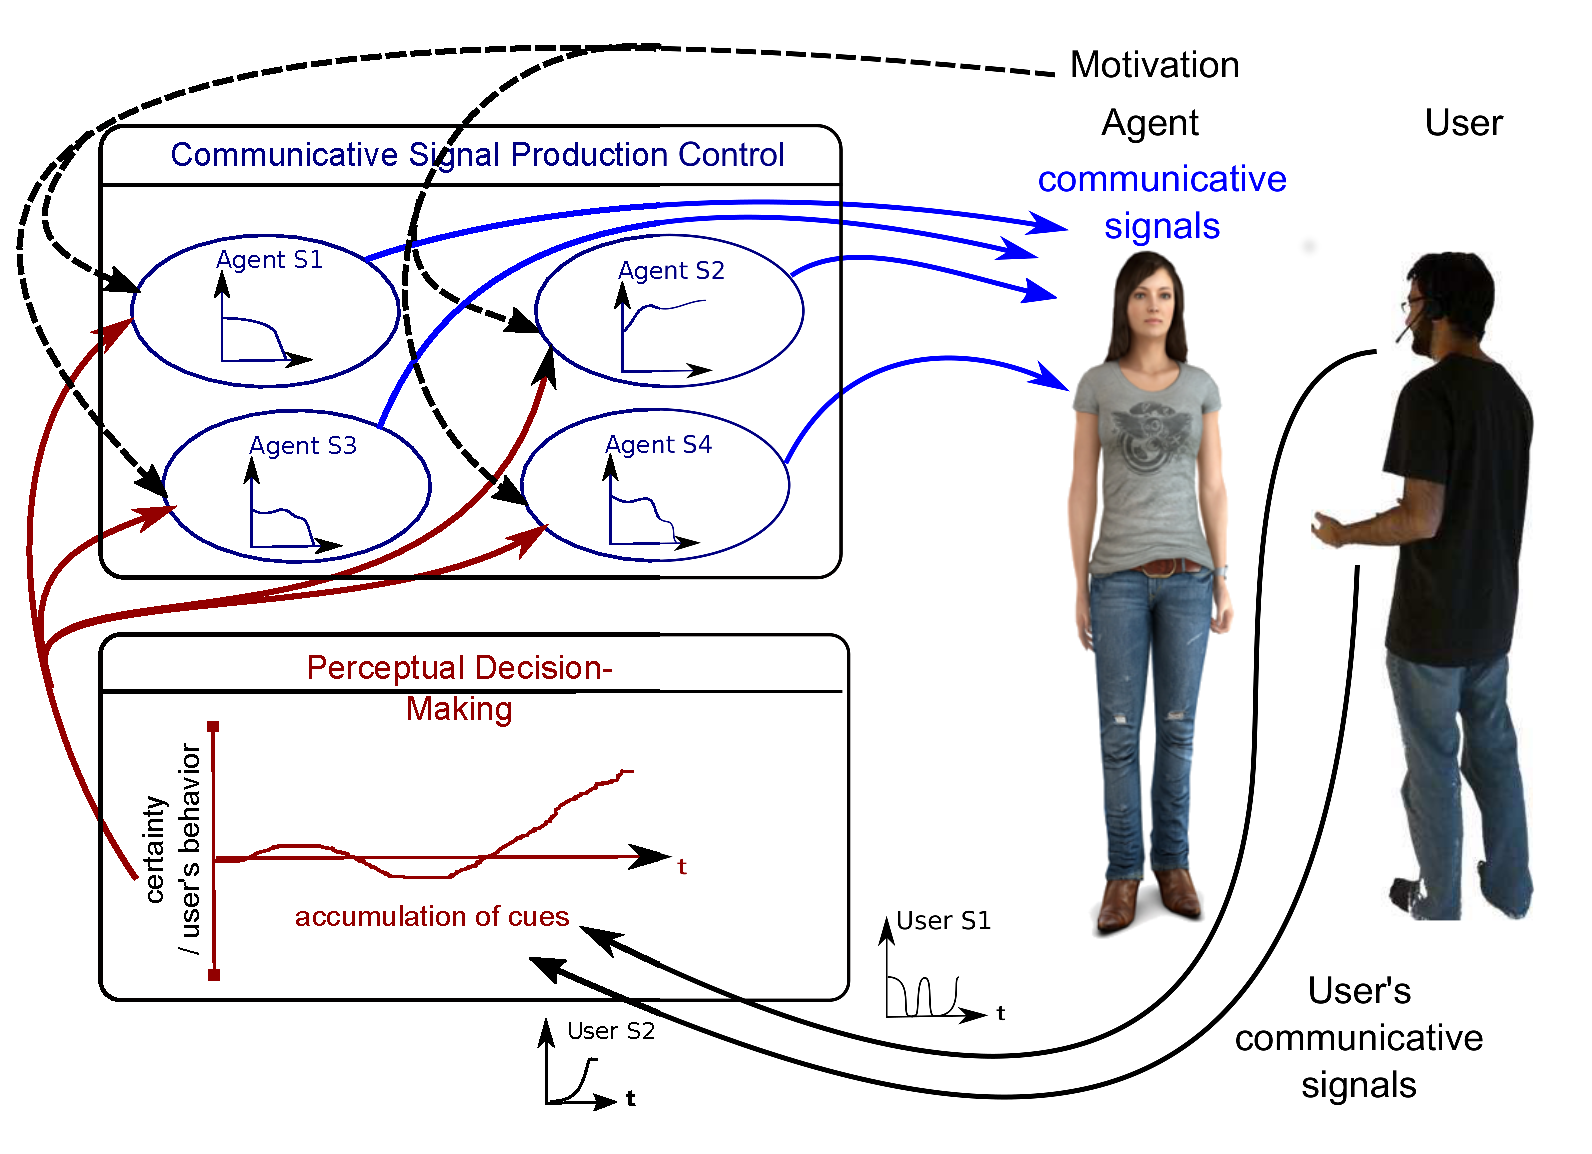
\includegraphics[width=\linewidth]{figure/modele_conceptuel_act.eps}
  \caption{Overview of the components of the theoretical model.}
  \label{fig:mod-comp}
\end{figure}

\subsubsection{Perceptual decision making}

This component accounts for the dynamics of the decision-making process. The underlying cognitive process is a perceptual decision-making task. The agent continuously perceives the variations in the signals produced by the user during the interaction, and it continuously evaluates its certainty about the willingness of the user to be the next speaker (or listener). This degree of certainty is represented by an accumulation variable (see Figure \ref{fig:mod-comp}).
The user behavior perception component follows the paradigm of Two Alternative Forced Choice (TAFC) tasks, for which different solutions have been proposed to model the timing of the decision-making process (see \citep{bogacz_physics_2006} for a review). 
The Drift Diffusion Model (DDM) has shown its ability to predict the time required by a human subject to accurately discriminate the nature of the information that it perceives for many tasks requiring perceptual decision making. 
Interestingly, the DDM has been used both in settings where the stimuli presented to the subject remained the same over the course of the decision-making process and in settings where the stimuli varied \cite{ratcliff_note_1980}. This model conceptualizes the dynamics of the agent's decision-making process as a stochastic process driven by the following equation:

\begin{equation}
  \frac{d\gamma(t)}{dt}=\alpha(t)+c\times\frac{dW}{dt}
  \label{perc_int}
\end{equation}

In our model, Equation \ref{perc_int}, $\gamma(t)$ represents the current degree of certainty that the agent has about the behavior of its partner, $\alpha(t)$ is an accumulation rate that varies with the user's signals, and $c\times\frac{dW}{dt}$ represents a noise in the perception process of the participants as defined by the DDM. The decision-making process is therefore continuously driven by the perception of the signals produced by the agent's partner.

The sign of $\gamma(t)$ indicates that the agent is tending to adopt one alternative or the other. 
When $\gamma(t)>0$, a higher value indicates that an agent is more certain about its partner's willingness to switch to the opposite role.
When $\gamma(t)<0$, a high absolute value means that the agent is very certain that its partner actually wants to keep its current role. 

The ongoing decision-making process ends when $\gamma(t)$ crosses a threshold $\theta_{\gamma}^{\pm}$. $\gamma(t)$ is then set to 0, and a new decision-making process starts.
$\gamma(t) \geq \theta_{\gamma}^{+}$ means that the agent is certain that its partner has switch to the opposite role, and the agent changes its behavior accordingly (defined by the component responsible for the control of signals). $\gamma(t) \leq \theta_{\gamma}^{-}$ means that the signals that it can perceive indicate that its partner wants to keep its current role. 
We will see in Section \ref{mod_analysis} that reinitializing this accumulation value allows, for instance, an agent motivated to take or yield the turn to attempt to initiate a new turn transition if the previous attempt did not succeed. 
This occurs when its partner does not respond to its turn-yielding signals by taking the turn  or when the agent's partner, being the current speaker, prevents the agent from taking the turn.

To account for the sensorimotor coupling between the two agents, we made the accumulation rate $\alpha(t)$ a function of the variations in the signals produced by the agent's partner. This function has a general shape defined by the following equation: 

\begin{equation}
  \alpha(t) = \sum_{j=0}^{n_{s}} \alpha_{j}(\dot{s}_j(t),s_j(t))
  \label{alpha_func}
\end{equation}

Equation \ref{alpha_func} means that $\alpha(t)$ continuously varies according to a sum of partial accumulation processes $\alpha_{j}$ that compute an accumulation rate for each signal $s_j$ that the agent can perceive ($n_s$ denotes the number of signals). %of the agent's partner. 
$\alpha_{j}>0$ indicates that the current variations in the signals produced by its partner are in favor of the assumption that the partner is switching to  the opposite role.
$\alpha_{j}<0$  means that the perceived variations in the signals are in favor of the assumption that the partner is keeping its current role. 

\paragraph{Illustrative simulation S1.}
Let us consider a situation consisting of an agent able to perceive the variations in loudness, pitch, and gaze direction of the user, three cues that are considered as used by participants to coordinate their turns (see section \ref{backgd}). 
In this simulated interaction, the agent was the current speaker, and the user was the current listener. The behavior of the user was simulated here.
The user averted its gaze after 750~ms and started to speak at $t=1~s$.
Figures \ref{fig-volume-user1}, \ref{fig-pitch-user1} and \ref{fig-gaze-user1} illustrate the variations in the simulated user's signal production, as perceived by the agent. 
Figure \ref{acc_example} illustrates the resulting dynamics of the perceptual decision-making process. 
The curve at the top is the evolution of the accumulation rate over time $\alpha(t)$, and the curve at the bottom is the evolution of the accumulation value $\gamma(t)$. In these scenarios, the second term, $c \times \frac{dW}{dt}$, has been set to 0 so that the accumulation process in this example has no noise. 

\begin{figure}
  \centering
  \includegraphics[width=\linewidth]{figure/loudness_simulated_partner.pdf}
  \caption{Illustrative simulation S1: variation in the voice loudness of the simulated user.}
  \label{fig-volume-user1}
\end{figure}

\begin{figure}%[b]
  \centering
  \includegraphics[width=\linewidth]{figure/Pitch_partenaire.pdf}
  \caption{Illustrative simulation S1: variation in the pitch of the simulated user.}
  \label{fig-pitch-user1}
\end{figure}

\begin{figure}
  \center
  \includegraphics[width=\linewidth]{figure/Gaze_partenaire.pdf}
  % \end{subfigure}
  \caption{Illustrative simulation S1: variation in the gaze direction of the simulated user.}
  \label{fig-gaze-user1}
\end{figure}

\begin{figure}
  \centering
  \includegraphics[width=\linewidth]{figure/illustration_ddm_speaker.pdf}
  \caption{Illustrative simulation S1: resulting dynamics of the perceptual decision-making process for the simulated speaker agent.}
  \label{acc_example}
\end{figure}

At the beginning of the scenario, the user did not produce any turn-taking signals; thus, $\gamma(t)$ was decreasing, meaning that the agent was becoming increasingly more confident about the user's intention to not claim the turn. 

At $t=0.75~\text{s}$, the agent started to obtain some information about the user's willingness to take the turn (gaze aversion); thus, the accumulation rate was positive. 
As soon as the user produced an additional turn-taking signal (starting to speak, resulting in a sudden increase in the pitch and volume of his voice), the accumulation rate increased. 
After $=1.2~\text{s}$, the user's gaze direction led the agent to believe that the user did not want to become the speaker, contradicting the information provided at that time by the verbal channel (the user was actually speaking). Therefore, the accumulation rate decreased to an intermediate positive value. 
As a result, the agent accumulated information about the user's intention to effectively take the turn, and $\gamma(t)$ reached the positive threshold ($\theta_{\gamma}^{+}=1$), leading it to be certain about the user's behavior. At this point ($t=4~\text{s}$), the agent made a definitive decision and reset its perceptual decision-making process. 

The  difference in the dynamics of the perceptual decision-making process, before and after $t=1~\text{s}$, illustrates the principle of the additivity of the perceptual decision-making process, captured by Equation \ref{alpha_func}: the more signals the user produces,
 the higher is the accumulation rate and the faster the agent detects that the user is taking the turn. This additivity of the perceptual process has been reported for human conversations \citep{gravano_turn-taking_2011,hjalmarsson_additive_2011}. 

\subsubsection{Production of the communicative signals}

The second component of our theoretical model controls the continuous production of the verbal and non-verbal signals of the agent.
Following the principles of the behavioral dynamics formulated by \citep{warren_dynamics_2006}, each signal produced by the agent is controlled by a differential equation, representing the law of control of the agent's behavior. These equations have the following general shape: 

\begin{equation}
  \ddot{a_j}(t)= -b\times\dot{a_j}(t) - k_g \times(a_j(t) - f(m(t),\gamma(t)))
  \label{signal_control}
\end{equation}

$a_j(t)$ represents the current value of signal $j$ ($\ddot{a_j}(t)$ being the second derivative of the signal), $-b$ is a damping term representing the intrinsic inertia of the agent to vary its signals, and $k_g\times(a_j(t)-f(m,\gamma))$ defines the value toward which the agent's signal is converging. In our theoretical model, each signal variable $a_j(t)$ is normalized to $ [0.0,1.0] $, with $0.0$ representing the minimal value of the signal (no-signal or baseline) and $1.0$ being the maximal value of the signal. The method with which these theoretical values are translated into realistic physical values depends on the nature of the signal and on the actuator used to execute the action corresponding to the signal produced. 
$k_g$ represents a stiffness parameter of the equation: a larger value of $k_g$ indicates that a participant will more rapidly vary its signal toward the final value of the equation. 
$f(m,\gamma)$ is a function that defines the attractor of the system. As presented at the end of Section \ref{backgd}, the modulation of each signal is directly influenced by the motivation of the agent, $m$, and the accumulation value $\gamma$ provided by the perceptual decision-making component of our model.

\paragraph{Illustrative simulation S2.} Let us consider an agent currently being the speaker and modulating two prosodic signals ($v$ = loudness, $p$ = pitch) and its gaze direction, $g$. 
Similar to the previous example, these variations are theoretical here.
The aim here was not to  exactly reproduce the variations in the signal observed during human conversations but rather to capture the dynamics of the signal productions, for instance, in that loudness and pitch tend to increase %and the speech rate to decrease 
during conflicting overlaps between partners and decrease during ends of turns. 

For each signal $j \in \lbrace p,v,g \rbrace$ produced by the agent, being the current speaker, we defined the following different equations $f_{j_{loc}}(m,\gamma)$, used in Equation \ref{signal_control}.
These functions dynamically control the value toward which each signal is varying at a given instant of time.

\begin{equation}
\begin{array}{lcl}
f_{p_{loc}} & = &  \frac{1}{2}\Big( 1 - S(\gamma) \big( \gamma m S(-m) - S(m+\gamma)S(m) \big) \Big)
%0.5 -0.5 \times \gamma \times m \times S(-m) \times S(\gamma) - 0.5 S(m+\gamma) \times S(\gamma) \times S(m)\\
 %& = & \frac{1}{2}(1 - S(\gamma)\times\gamma \times m \times S(-m) - S(m+\gamma) \times S(m)))
\end{array}
\label{eq_speaker_pitch}
\end{equation}

\begin{equation}
f_{v_{loc}} = f_{p_{loc}}
\label{eq_speaker_volume}
\end{equation}

\begin{equation}
\begin{array}{lcl}
f_{g_{loc}}&=& \frac{1}{2}\Big( 1+\gamma m S(\gamma) \big(S(m) - S(-m)\big) \Big)\\
%& & 0.5 +0.5\times \gamma \times m \times S(\gamma) \times S(m) \\
%& & -0.5 \times \gamma \times m \times \times S(\gamma) \times S(-m) \\
%&=& \frac{1}{2}((1+\gamma \times m \times S(m) \times (S(\gamma) - \gamma \times m \times S(\gamma) \times S(-m))\\
\end{array}
\label{eq_speaker_gaze}
\end{equation}

\begin{equation}
S(x) = \frac{1}{1+e^{-10x}}
\label{eq_sigmoid}
\end{equation}

In these equations, we used the sigmoid function $S$ (Equation \ref{eq_sigmoid}), which permits us to set some terms to $0$, depending on the value of $\gamma(t)$ or $m(t)$ (when $x \gg 0$, $S(x)\approx 1$, and when $x \ll 0$, $S(x)\approx 0$). 
For example, for the control of the pitch,  when $m(t) \gg 0$, Equation \ref{eq_speaker_pitch} reduces to $f_{p_{loc}}(m,\gamma) \sim \frac{1}{2}\big( 1-S(\gamma) \big)$, 
when $m(t) \ll 0$, $f_{p_{loc}}(m,\gamma) \sim \frac{1}{2}\big( 1 + S(\gamma)\big)$ 
and when $\gamma(t) \ll 0$, $f_{p_{loc}}(m,\gamma) \sim \frac{1}{2}$. 

We set these functions such that when the current speaker has a strong motivation to continue speaking ($m(t) \ll 0$) and has accumulated enough cues indicating that the current listener is about to take the turn  ($\gamma(t) \gg 0$), the agent is expected to increase the loudness and pitch of its voice to avoid its partner from taking the turn, resulting in a conflicting overlap. 
On the other hand, when the current speaker's current goal is to leave the turn ($m(t) \gg 0$), the speaker is expected to lower its loudness and pitch, even faster if the listener is starting to speak (all the signals are decreasing to 0).
Notice that setting $f_p = f_v$ is an approximation that makes the two signals follow the same dynamics according to the signs of $m(t)$ and $\gamma(t)$. 

Because our approach assumes the sensory-motor coupling of the two interacting agents, here, we have to simulate the dynamic of its partner's behavior, as perceived by the agent.
For the sake of simplicity, we simulated the dynamic of the perceptual decision making using the following equation: $\gamma(t)=1-2e^{-t}$. 
This means that in our simulated scenario, the agent was initially certain that the listener was not claiming the turn ($\gamma(0) = -1$) and that the agent was rapidly accumulating some cues concerning the current listener's behavior indicating the willingness of the listener to take the turn. 

Figure \ref{demo_simu_l1} shows how the agent varied its prosodic signals when it was strongly motivated to continue speaking ($m=1$).
As the accumulation $\gamma(t)$ increased, the resulting values of $f_v$ and $f_p$ increased toward $1$, and $f_g$ decreased toward $0$. 
Accordingly, the theoretical loudness and pitch of the agent increased to their maximum values (as expected during a conflicting overlap where the speaker attempts to maintain its role and thus is modulating its signal production) in reaction to the behavior of the listener who was attempting to take the turn. 

\begin{figure}
  \centering
  \includegraphics[width=\linewidth]{figure/signals_simu_s2a.pdf}
  \caption{Illustrative simulation S2: time series of the simulated speaker's signal productions. (a) Simulation of the agent's perceptual decision-making process (value of $\gamma$). (b) The variations in $f_v(m,\gamma)$, $f_p(m,\gamma)$, and $f_r(m,\gamma)$ . (c) Resulting  signal productions. Case of an agent with a very strong motivation to continue being the current speaker ($m=-1.0$).}
  \label{demo_simu_l1}
\end{figure}

To illustrate how the agent's motivation impacts the dynamics of the signal production, we simulated the same scenario but with a speaker motivated to yield the turn ($m=1$). As illustrated in Figure \ref{demo_simu}, in this case, $f_v$ and $f_p$ both decreased toward $0$, leading to a variation in the theoretical loudness and pitch toward $0$ and illustrating a situation in which the agent yielded the turn, as it also perceived that the listener was taking the turn. 

\begin{figure}
  \centering
  \includegraphics[width=\linewidth]{figure/signals_simu_s2b.pdf}
  \caption{Illustrative simulation S2: time series of the simulated speaker's signal productions. (a) Simulation of the agent's perceptual decision-making process (value of $\gamma$). (b) The variations in $f_v(m,\gamma)$, $f_p(m,\gamma)$, and $f_r(m,\gamma)$ . (c) Resulting  signal productions. Case of an agent with a very strong motivation to leave the turn ($m=1.0$).}
  \label{demo_simu}
\end{figure}

\section{Properties of the theoretical model}
\label{mod_analysis}

In Section \ref{mod_pres}, we have presented separately the two components of our theoretical model. 
We now want to show the relevance of the model for the coordination of speech turns in user-agent interactions.
We demonstrate how the model accounts for the basic features of the interpersonal coordination between participants, namely, the capacity to coordinate their turns in various situations, when the agents have compatible goals as well as when they are temporarily in conflict. In the first case, smooth transitions occur, whereas in the latter, conflicting overlaps remain limited.
Then we will show how the model allows the agent to adapt its behavior according to the amount of information it can obtain about the user's behavior.
All these properties result from the coupling in the signal production of the two interacting participants: the instantaneous behavior of the agent (its signal production) results from the interplay between the variation in its own motivation, with respect to its role in the conversation (speaker versus listener), and its ongoing perceptual decision-making process. 
As a result, the coordination emerges from the interaction between participants, without the support of any explicit algorithm or set of rules.
This emergence comes from the nature of the equations of the two components of the model (Equations \ref{perc_int}, \ref{alpha_func} and \ref{signal_control}). 

\subsection{Equations}

As in the previous section, we simulated the interaction between an agent and a hypothetical user. For the sake of clarity, let us consider that the agent is the current speaker and that the user is the current listener; however, of course, the opposite configuration would give the same results. In this simulated scenario, both the agent and the user produced and perceived the same set of signals: volume and pitch of the voice and gaze direction, resp. $v,p,g$.

\subsubsection{Equations of the perceptual decision-making process}

Tables \ref{acc_functions_speaker} and \ref{acc_functions_listener} give the functions that correspond to the different components of Equation \ref{alpha_func} when the agent is the speaker and the listener, respectively. 
The basic assumption is that each signal perceived by the agent provides some cues about the willingness of its partner to maintain or leave its current role. It is worth noting that these cues may be temporarily congruent or in apparent contradiction.
We set these partial accumulation functions such that the agent interprets similar signals variations, as we observe in human conversations. For a listener agent, values of loudness and pitch being less than $0.4$ and the partner looking toward the agent (gaze value of greater than 0.5) are end-of-turn cues, whereas loudness and pitch values being higher than $0.5$ and a speaker averting its gaze (gaze value of less than 0.5) from the agent are better associated with turn keeping. For a speaker agent, the values of loudness and pitch indicating that the user is starting to speak (in our example higher than $0.1$) and averting his gaze (gaze value less than 0.5) from the agent are turn-taking cues.

\begin{table}
\centering
\begin{tabular}{|c|c|c|}
\hline
Cue & Speaker \\
\hline
Loudness & $\alpha_{v_{loc}}(v,\dot{v})=1.5\times (v-0.1)$ \\
\hline
Pitch & $\alpha_{p_{loc}}(p,\dot{p})=1.5\times (p-0.1)$ \\
\hline
Gaze & $\alpha_{g_{loc}}(g,\dot{g})=-1.5\times (g-0.5)$ \\
\hline
\end{tabular}
\caption{Set of accumulation functions used in Equation \ref{alpha_func} for the speaker.}
\label{acc_functions_speaker}
\end{table}

\begin{table}
\centering
\begin{tabular}{|c|c|c|}
\hline
Cue & Listener \\
\hline
Loudness & $\alpha_{v_{lis}}(v,\dot{v})=-2.0\times (v-0.4)$ \\
\hline
Pitch & $\alpha_{p_{lis}}(p,\dot{p})=-2.0\times (p-0.4)$ \\
\hline
Gaze & $\alpha_{g_{lis}}(g,\dot{g})=1.0\times (g-0.5)$ \\
\hline
\end{tabular}
\caption{Set of accumulation functions used in Equation \ref{alpha_func} for the listener.}
\label{acc_functions_listener}
\end{table}

\subsubsection{Equations of signal production}

For the simulation of the speaker's behavior, we used the set of Equations \ref{eq_speaker_pitch}, \ref{eq_speaker_volume}, \ref{eq_speaker_gaze} and \ref{eq_sigmoid}. Figures \ref{fig_pro_loc} and \ref{fig_gaze_loc} represent the resulting values of $v_{loc}$, $p_{loc}$ and $g_{loc}$, computed using Equation \ref{signal_control}.

\begin{figure}
\centering
\includegraphics[width=\linewidth]{figure/bifurcProsodyLoc.pdf}
\caption{Values of $v_{loc}$ and $p_{loc}$ as functions of $m(t)$ and $\gamma(t)$.}
\label{fig_pro_loc}
\end{figure}

\begin{figure}
\centering
\includegraphics[width=\linewidth]{figure/gazeLoc.pdf}
\caption{Values of $g_{loc}(m,\gamma)$}
\label{fig_gaze_loc}
\end{figure}

For the listener, the functions governing the variation in the attractor of Equation \ref{signal_control} are as follows:
 
\begin{equation}
f_{v_{lis}}= f_{p_{lis}} = \frac{1}{2} \gamma S(m+\gamma) + S(m+\gamma)S(m)S(-\gamma)
\label{lis_pro}
\end{equation}

\begin{equation}
f_{g_{lis}} = 1 - S(m + \gamma)
\label{lis_gaze}
\end{equation}

These equations have been defined such that when the speaker does not produce cues, the values of the loudness and pitch equal $0$, and the gaze value equals $1$; the listener is silent and constantly fixing its gaze toward the speaker. 
According to these equations, when $m(t)<0$, $\gamma(t)>0$, and $|\gamma(t)|>|m(t)|$ or when $m(t)>0$, $\gamma(t)<0$, and $|\gamma(t)|>|m(t)|$, the listener will attempt to grab or take the turn by increasing its loudness and pitch values and averting its gaze from the current speaker. Figures \ref{fig_pro_lis} and \ref{fig_gaze_lis} illustrate the distribution of the attractors of Equation \ref{signal_control} using Equations \ref{lis_pro} and \ref{lis_gaze}.

Figures \ref{fig_pro_loc} to \ref{fig_gaze_lis} illustrate the dynamic interplay between the agent's intrinsic motivation and the influence of the agent's partner behavior.
During the interaction, $m$ and $\gamma$ are continuously varying, which results in the continuous modulation of the agent's prosodic and non-verbal signals productions. Because the $\gamma$ of each agent depends on the signals $s_j$ produced by the other agent, the model accounts for the coupling of the two agents. This coupling makes the agent's non-verbal signals follow an emergent trajectory. The next section illustrates how the turn-taking behavior, and more generally the coordination, emerges from these complex dynamics. 

\begin{figure}
  \centering
  \includegraphics[width=\linewidth]{figure/bifurcProsodyLis.pdf}
  \caption{Values of $v_{lis}(m(t),\gamma(t))$ and $p_{lis}(m(t),\gamma(t))$}
  \label{fig_pro_lis}
\end{figure}

\begin{figure}
  \centering
  \includegraphics[width=\linewidth]{figure/gazeLis.pdf}
  \caption{Values of $g_{lis}(m(t),\gamma(t))$}
  \label{fig_gaze_lis}
\end{figure}

\subsection{Emergence of behavior}

In the previous section, we analyzed the dynamics of the state variable $\gamma$ as a response to the agent's intrinsic motivation $m$, which acts as a forcing variable in our model. In this section, we explain how the two agents coordinate their speech turns in various situations, although they are not endowed with any explicit coordination algorithm. We show that the model accounts for the different situations observed in human conversations and that the moment of time at which the transition of turns occurs or how long competitive overlaps last is  controlled by any specific agent; rather, it dynamically emerges from the interaction. Indeed, we illustrate this emergence through three contrasting scenarios, summarized in Table \ref{tab_scenarios_emergence}, that show that varying the motivation of only one of the two participants strongly changes the behavior of the other participant. For the sake of demonstration, in these simulations, the agents' motivation remained constant during the whole interaction. 

\begin{table}
  \begin{center}
    \begin{tabular}{ccc}
      \hline
      \mbox{} & Speaker's goal, $G_{loc}$ & Listener's goal $G_{lis}$\\
      \hline
      S3 & opposite, $m=1.0$ & strong, $m=1.0$\\
      \hline
      S4 & strong, $m=-1.0$ & strong, $m=1.0$\\
      \hline
      S5 & strong, $m=-1.0$ & low, $m=0.15$\\
      \hline
    \end{tabular}
  \end{center}
  $G_{loc}$: go on speaking (keep the same goal)\linebreak
  $G_{lis}$: say something (change to the opposite role)

  \caption{Scenarios for the analysis of the emerging behavior. Values of the forcing variable $m$ for the two agents.}
  \label{tab_scenarios_emergence}
\end{table}

\begin{figure}[b]
  \centering
  \includegraphics[width=\linewidth]{figure/smooth-transition_signal-production.pdf}
  \caption{Modulation of the verbal and non-verbal signals produced by the two agents. The resulting behavior is a smooth transition of the turn from the current speaker to the current listener. Scenario S3} 
  \label{simu_smooth}
\end{figure}

\begin{figure}[t]
  \centering
  \includegraphics[width=\linewidth]{figure/smooth-transition_accumulation_small.pdf}
  \caption{Time series of the accumulation values $\gamma$ for the two agents. Scenario S3.}
  \label{smooth_acc}
\end{figure}


In scenario S3, the current speaker had a strong motivation to become the listener, and the current listener had a strong motivation to become the speaker. Figure \ref{simu_smooth} shows how the agents modulated their prosodic and non-verbal signal productions (here, the loudness and pitch of their voice as well as their gaze direction). Figure \ref{smooth_acc} shows the dynamic of the perceptual decision-making process. As one could expect, the model led to a short non-conflicting overlap, in the terms given by \citep{schegloff_overlapping_2000}. 

Scenario S4 shows that if we modify the current speaker's motivation, we impact the behavior of the two agents. In S4, the current speaker had a strong motivation to continue speaking, and the current listener had a strong motivation to become the speaker. The result of this simulation is shown on Figure \ref{simu_interruption} and  Figure \ref{inter_acc}. In this situation, the model reproduced a conflicting overlap, which ended with the initial listener having the floor.  

\begin{figure}
  \centering
  \includegraphics[width=\linewidth]{figure/emerg_sc1.pdf}
  \caption{Modulation of the prosodic and non-verbal signals produced by the two agents. Scenario S4. The resulting behavior is a conflicting overlap lasting approximately 2 seconds.}
  \label{simu_interruption}
\end{figure}

\begin{figure}
  \centering
  \includegraphics[width=\linewidth]{figure/acc_sc4_small.pdf}
  \caption{Time series of the accumulation values $\gamma$ for the two agents. Scenario S4.}
  \label{inter_acc}
\end{figure}

This scenario shows the continuous dependency of each participant on the production of signals by the other participant. At the beginning of the simulation, the current speaker was maintaining its voice loudness as its mean value of $0.5$. As its accumulation value increased, due to the increase in the loudness and pitch of the current listener, at $t\approx~750~\text{ms}$, the current speaker increased its own prosodic variables and averted its gaze, demonstrating to the current listener its willingness to remain the speaker. Nevertheless, the modulations of the current speaker's signals (as defined by the equations governing the production of signals) weakly impacted the current listener's the production of signal. As a result, the current listener continued to attempt to grab the turn, the accumulation value of the current speaker crossed the positive threshold, and the current speaker finished, thereby releasing the turn to the current listener. Subsequently, the current listener diminished its loudness and pitch, perceiving that the previous speaker finished to release the turn, which finally ended the conflictual situation.

If we now keep the same motivation value for the current speaker but diminish the motivation of the current listener, we obtain a completely different behavior for the two agents, as shown by Figures \ref{simu_buttin} and \ref{acc_buttin}, corresponding to scenario S5. We illustrate here the listener's successive but unsuccessful attempts to grab the turn. The choices made in the specific equations used for these simulations are responsible for how the conflict is resolved here.  

\begin{figure}
  \centering
  \includegraphics[width=\linewidth]{figure/emerg_sc2.pdf}
  \caption{Modulation of the prosodic and non-verbal signals produced by the two agents. Scenario S5.}
  \label{simu_buttin}
\end{figure}

\begin{figure}
  \centering
  \includegraphics[width=\linewidth]{figure/acc_sc2_small.pdf}
  \caption{Time series of the accumulation values $\gamma$ for the two agents. Scenario S5.}
  \label{acc_buttin}
\end{figure}

In S5, the current speaker succeeded in maintaining its role despite the several turn-taking attempts made by the current listener. This was because the motivation of the current listener was weaker than before, meaning that it gave up more easily when it observed no cues indicating that the current speaker was releasing the turn. At the beginning of the simulation, the accumulation value of the current speaker increased, resulting in a current speaker averting its gaze from the listener. When the current listener gave up, the accumulation value of the current speaker diminished again, resulting in a gaze control parameter returning to the value $s_g=1$, meaning that the agent was fixing its partner. The fact that the loudness and pitch did not vary was simply due to an accumulation that was not high enough for the prosodic signals to increase. In other words, the agent did not need to increase its prosodic signals to prevent the current listener from grabbing the turn. The observed repetition of the turn-taking attempts of the current listener was due to the fact that, as defined in Section \ref{mod_pres}, when the accumulation value crosses the negative threshold, the accumulation process is reinitialized. Thus, the current listener again became  uncertain about the behavior of the current speaker and thus initiated a new turn-taking attempt. 


These three simulations show that the resulting behavior of each participant is not solely determined by their motivation value but rather is also indirectly impacted by the motivation of the other participant. In this sense, a sensorimotor coupling is established between participants, as the action variations by one participant directly impact the modulation of the actions of the other participant, resulting in a very versatile coordination. Because both participants continuously influence the other participant's behavior, one cannot predict in advance the resulting behavior of the two participants. These behaviors are thus an emergent property of the interaction of the two participants. 

\subsection{Adaptability of the behavior}

The behaviors of the two participants emerge from the interaction. However, what benefits are produced by this sensorimotor coupling between both participants?
We show in this section that this sensorimotor coupling can explain how participants can seamlessly adapt to different environmental settings without modifying the different equations governing the perceptual decision-making process and the production of the prosodic and non-verbal signals. We will show this adaptability using examples in which we varied the number of signals that the agents can perceive. 

The different analyses conducted in this section have been performed using scenario S5 (see Table \ref{tab_scenarios_emergence}) and a variant, S6, where the agents did not use the direction of the gaze of their partner in the perceptual decision-making process. 
These two scenarios correspond to a conflicting situation whereby when the current listener makes several unsuccessful attempts to grab the turn, the current speaker averts its gaze in response to the turn-grabbing attempt. Figure \ref{simu_buttin} illustrates the signal production of the two participants when they perceived the totality of the signals produced by the other participant (S5). Figure \ref{adapt_nogaze} illustrates what occurred when the agents did not have access to the gaze direction of their partner (S6).

\begin{figure}
  \centering
  \includegraphics[width=\linewidth]{figure/adapt_nogaze.pdf}
  \caption{Conflictual situation where the participants do not have access to the gaze information of the other participant. Scenario S6.}
  \label{adapt_nogaze}
\end{figure}

In scenario S5, where participants exchanged the whole set of signals, the speaker's accumulation value increased but remained negative as the current listener attempted to grab the turn but rapidly gave up. This was because the information conveyed by the listener's gaze evolved more slowly than the prosodic information. Thus, initially, the speaker did not perceive the cue in the gaze information indicating that the listener wanted to grab the turn,  consequently diminishing the variation in the accumulation value. 

In scenario S6, the accumulation value of the listener increased more rapidly and took more time to decrease in response to the lack of cues indicating that the speaker released the turn, resulting in an agent further increasing its loudness and pitch for longer durations. The fact that the loudness and pitch of the listener increased also more strongly impacted  the accumulation value of the speaker that increased further and became positive, which was not the case previously, resulting in an agent that further increased its own loudness and pitch. This increase impacted the accumulation value of the listener, which decreased again, resulting in the listener giving up its turn-taking attempt. 

In addition, we simulated a situation in which the participants perceived only the voice loudness, and we observed the same type of adaptation: the speaker further increasing  its loudness in response to the turn-taking attempts of the listener, as shown in Figure \ref{adapt_volume}.

\begin{figure}
  \centering
  \includegraphics[width=\linewidth]{figure/adapt_volume.pdf}
  \caption{Conflictual situation in which the participants have access only to the loudness produced by the other participant.}
  \label{adapt_volume}
\end{figure}

What is remarkable about these three contrasting scenarios is that the duration of the conflicts did not vary significantly with the number of signals handled by the agents. Interestingly, the participants kept the coordination effective, which was not explicitly defined in the equations but rather emerged from the manner in which the participants varied their signals, accentuating their signal productions to compensate for the lack of information in the environment. The adaptation of the agents is thus an emergent property of the interaction. Such mechanism is a great advantage for a turn-taking model between an agent and an user, as the adaptation of the agent is naturally done during the course of the interaction, without needing an explicit adaptation algorithm. Nevertheless, having the same adaptation properties in user-agent interactions necessitates that the user also be able to actively adapt to the situation. We explore this point in Section \ref{sec:eval}.

\section{Implementation of the model}
\label{impl}

\subsection{Requirements}

Turn-taking management is one of the many processes an ECA has to manage to be engaged in a natural interaction with the user. 
Among others, turn-taking management is closely linked with 
the dialog management, including natural language understanding and generation \citep{skantze_towards_2010}, 
grounding which necessitates the generation of and reaction to the different types of feedback that the user may produce, such as backchannels \citep{kopp_dynamic_2014,bevacqua_multimodal_2010}, 
and also the control of the engagement process with the user (see \cite{clavel_fostering_2016} for a review about engagement). 
Existing ECA architectures provide the core functionalities required to support these processes, at least partially. 
Our aim was to propose a solution for integrating our model into existing ECA architectures.
However, the continuous nature of the two main components of the model that are executed in parallel implies some adaptations of existing architectures. 

The closest solution suitable for implementing our model is ASAP from \cite{kopp_architecture_2014}.
Nevertheless, some mandatory details are lacking in the specifications of the ASAP architecture. For instance, we have to manage the concurrent execution of the different decision modules. Indeed, several conflicting actions can be sent to the realizer simultaneously, which thus requires a mechanism to select or merge the actions to avoid inconsistencies in the action generation. Another issue is the selection of the multimodal communicative actions corresponding to the commands provided by the decision modules and specifically how to handle commands that require  actions produced by the agent to be changed in real time. 
We borrowed some principles from the Ymir architecture \cite{thorisson_mind_1999} to address these issues and thus extended the ASAP architecture.  

\subsection{Architecture overview}

The overall organization of the BeAware architecture, which is composed of six modules, is similar to ASAP, as shown in Figure \ref{overall_archi}. 
The modules dedicated to  perception are 
the Sensing module receiving sensory data, 
the Behavior Interpreter module, which interprets behavioral patterns, such as nodding, from the multimodal sensory data, 
and the Function Interpreter, which interprets the communicative functions of the behavioral patterns. 
The decision part is composed of three modules:
the Intent Planner, which generates the communicative intentions of the agent; 
the Behavior Planner, which generates the multimodal actions from the communicative intentions and manages the execution of the actions (activating, modulating or interrupting the actions) based on the behavioral patterns perceived by the Behavior Interpreter;
and finally the Behavior Realizer. 

\begin{figure}
  \centering
  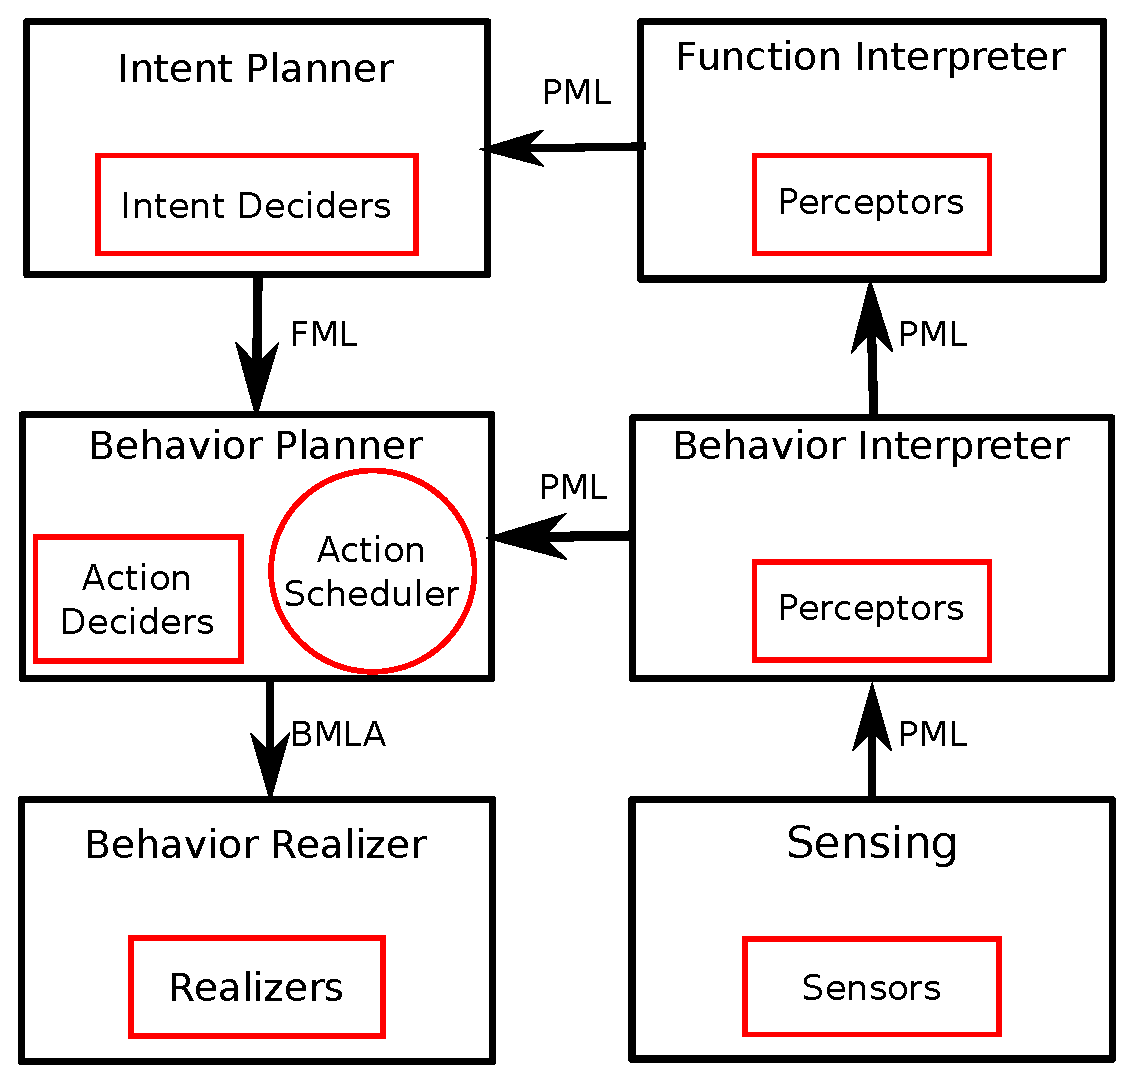
\includegraphics[width=\linewidth]{figure/impl_schema.eps}
  \caption{Overall organization of the BeAware architecture.}
  \label{overall_archi}
\end{figure}

Each module is compounded of submodules, each specialized as follows: \begin{itemize}
	\item the real-time acquisition of the user's verbal and non-verbal signals for the submodules of the Sensing Module;
	\item the perception of a particular behavioral pattern or communicative act for the submodules of the Behavior Interpreter and Function Interpreter;
	\item the generation of a particular communicative intention for the submodules of the Intent Planner;
	\item the control of a particular multimodal action for the submodules of the Behavior Planner; and
	\item the execution of particular BML commands for the submodules of the Behavior Realizer.
	\end{itemize}		
	Following the terminology of \cite{thorisson_mind_1999}, the submodules of the behavior and function interpretation modules were called perceptors, those of the Sensing modules were called the sensors, those of the Intent Planner and the Behavior Planner were called the deciders, those of the Behavior Realizer were called realizers, and the submodules of the sensing module were called the sensors.  
Following the Ymir principles, the different submodules run concurrently at their own execution frequency. 
As in Ymir, the submodules can also be either activated or deactivated. 
The activation or deactivation of modules depends on the current state of the dialog. 
For instance, modules implementing the equations of our model controlling the non-verbal signals of the speaker are activated only when the agent is in the Speaker state  and are deactivated when the agent is in the Listener  state. 
The activation or deactivation of the submodules is implemented in the Function interpreter module by so-called Module Managers. 

We distinguish two types of deciders: intention and action deciders. 
Intention deciders belong to the Intent Planner and are responsible for the generation of the communicative intentions based on the perception data provided by the function interpretation module. Intention deciders output FML data. 
The action deciders take as input the communicative intentions provided by the intention deciders as well as the perceptual data provided by the behavior interpretation module. As output, they generate an action command that describes the action to control and the new values of the action parameters according to the perceptual data and the agent's communicative intention. 
These commands are then sent to an action scheduler that is responsible for transcribing the commands into BML motor commands and managing their concurrent executions. Once the motor commands have been determined, the action scheduler sends them to the realizers. 
The design of our action scheduler is very similar to Ymir's action scheduler. The difference is linked to the management of the continuous multimodal actions: the deciders modulating the actions of the agent send a continuous flow of commands to the action scheduler. Our action scheduler manages this continuous flow of commands, with the capability of modifying the multimodal motor commands bound to a particular action on the fly, based on the parameters that the deciders send to the action scheduler. 
Finally, the action scheduler sends the different motor commands to the corresponding realizers using BML structures. 

\subsection{Implementation}

Figure \ref{impl_modules} illustrates how the different submodules are implemented in the architecture. 

\begin{figure}
  \centering
  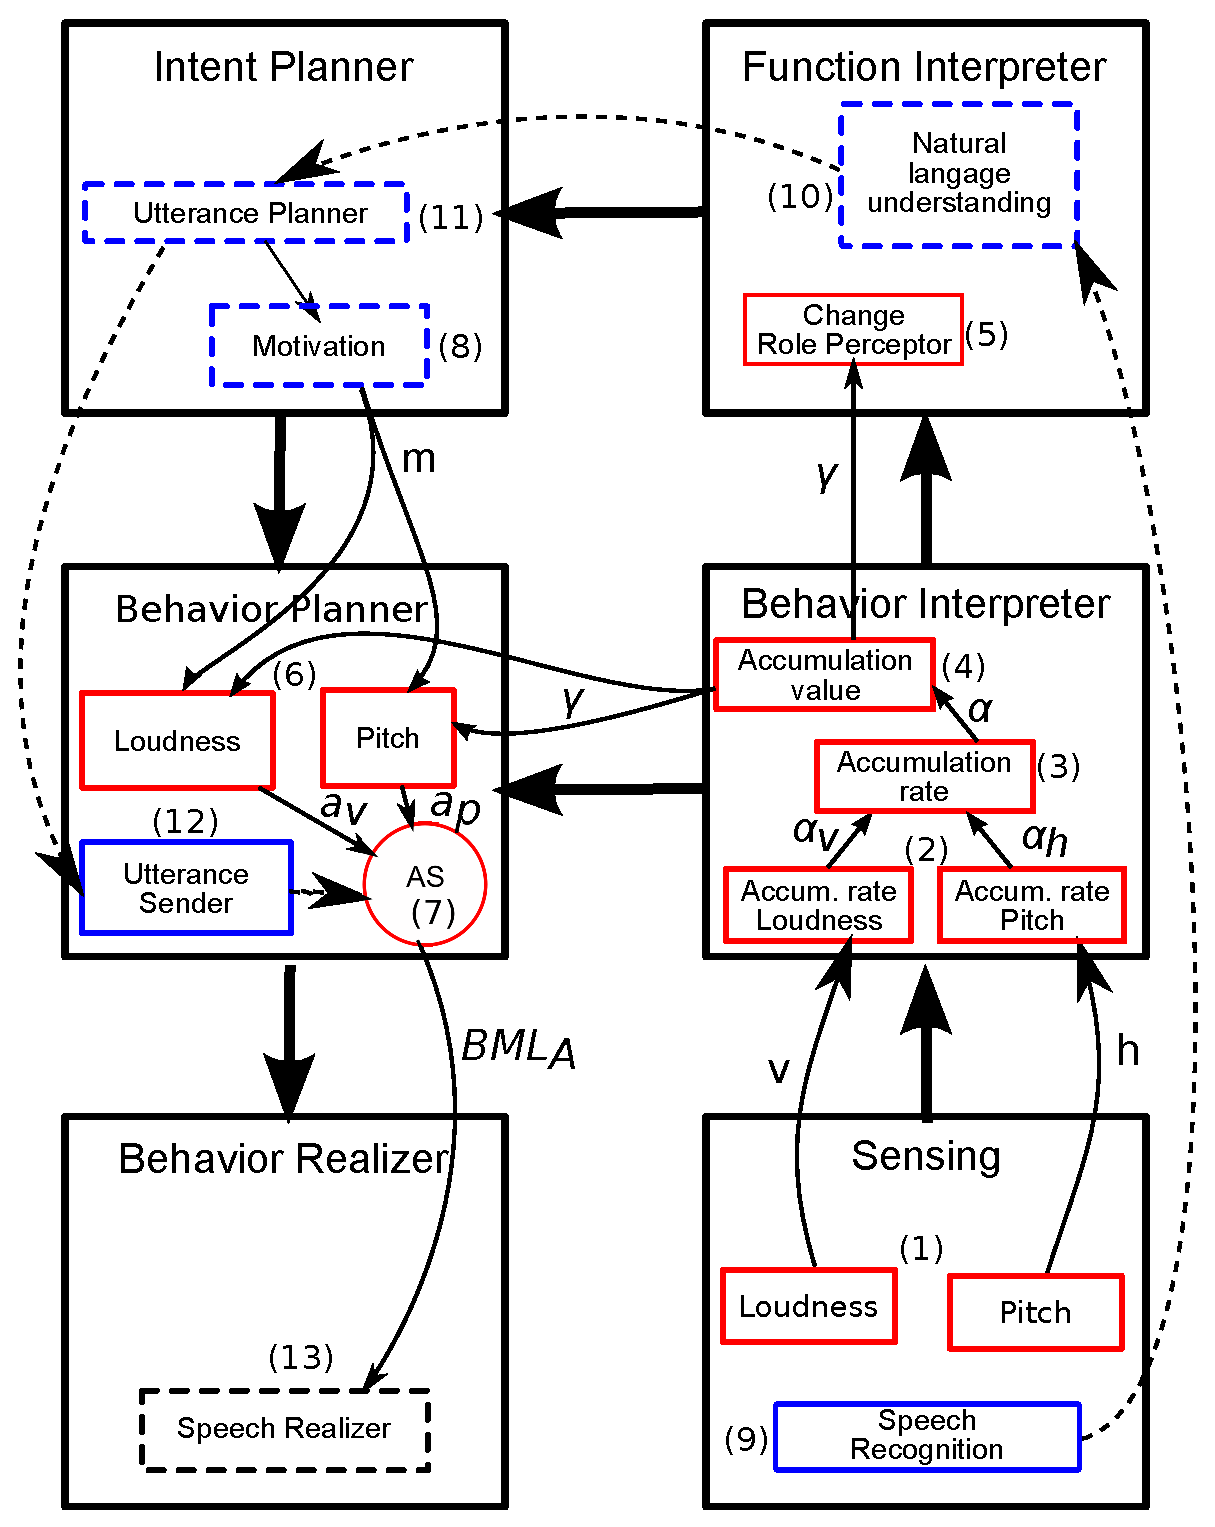
\includegraphics[width=\linewidth]{figure/impl_equ_dial.eps}
  \caption{Distribution of the components of the model and the different submodules dedicated to the utterance interpretation and generation as well as the determination of the motivation value.}
  \label{impl_modules}
\end{figure}

\subsubsection{Perceptual decision-making process}

According to our model, the agent is continuously collecting information about the user's behavior. This is done by submodules of the Sensing Module, indicated by (1) in Figure \ref{impl_modules}. Two submodules are currently implemented, the Loudness and Pitch submodules, which gather in real time the loudness and pitch of the current user. 

This information is a set of characteristics computed in real time from the data that the agent is able to sense, which are used to compute the accumulation rate $\alpha(t)$. 
Each partial accumulation function $\alpha_j(t)$ is evaluated in a separate submodule (modules indicated by the number (2) in Figure \ref{impl_modules}). The values computed by these modules are then summed by a dedicated perceptor ((3) in Figure \ref{impl_modules}) according to Equation \ref{alpha_func} and integrated by a final submodule ((4) in Figure \ref{impl_modules}), which computes the final accumulation value $\gamma$ according to Equation \ref{perc_int}). The final accumulation value is then transmitted to both the Behavior Planner and the Function Interpreter. The Function Interpreter implements a submodule ((5) in Figure \ref{impl_modules}) that evaluates the resulting accumulation value $\gamma$ and that is in charge of changing the agent's current state (speaker or listener) when $\gamma$ has crossed the positive threshold $\theta_{\gamma}^{+}$. As we define a different set of equations depending on whether the agent is the current speaker or the current listener in our model (see Sections \ref{mod_pres} and \ref{mod_analysis}), the agent has a different set of modules for the perception of the user's behavior and control of prosodic actions. Thus, when the agent has changed its state, the set of perception and control modules associated with its previous state are deactivated, and the set of perception and control modules associated with its next state are activated. 

\subsubsection{Modulation of the prosodic signals}

The corresponding components are implemented in the Behavior Planner ((6) in Figure \ref{impl_modules}). Each of these modules implements specific equations controlling the modulation of a particular signal according to the general shape of Equation \ref{signal_control}. Each action decider has two inputs: the motivation $m(t)$ to change role, originating from the Intent Planner, and the accumulation value $\alpha(t)$, originating from the Behavior Interpreter. 
Once the pitch and loudness values are computed, the deciders send these values to the action scheduler ((7) in Figure \ref{impl_modules}), which is in charge of transforming these commands into BMLA commands (an extension of BML introduced by \citep{kopp_architecture_2014}), which are then sent to the Realizers. 
In our current implementation, two deciders are currently implemented, one for pitch modulation and one for loudness modulation. 
The choice of independently control of the different signals may seem inconsistent, especially when separately controlling pitch and loudness. Indeed, when the loudness is equal to $0$, the agent does not produce any sound, and discussing pitch variation does not make sense. However, the equations of our model define the control parameters of the different realizers and do not correspond to the real signal values. Potential inconsistencies are then resolved later by the Realizer.  

\subsubsection{Management of the motivation}

The motivation to speak, or to listen, may be based on different factors. If the agent is finishing its utterance and has nothing more to say, its motivation to be the listener will be positive; otherwise, its motivation will be negative. The strength of this motivation is regulated by different processes, for instance, the interpersonal attitudes of the participants \citep{ter_maat_how_2010,ravenet_conversational_2015} or the importance and nature of the contribution made by the participant \citep{cafaro_effects_2016}. As the nature of the factors influencing the motivation to speak can be different, we chose to implement its computation in an independent module of the Intent planner ((8) in Figure \ref{impl_modules}). This module updates over time the motivation of the agent and then sends FML data specifying the new motivation value to the Behavior planner. 


\subsubsection{Verbal production}

In addition to the submodules implementing our turn-taking model, we added submodules dedicated to the interpretation of the user's utterances. 
A user's utterance is first perceived incrementally by the Speech Recognition Module ((9) in Figure \ref{impl_modules}) and is then  transmitted to the Natural Language Understanding module ((10) in Figure \ref{impl_modules}), which maps the user's utterance with a semantic value. This semantic value is then transmitted to the Utterance Planner ((11) in Figure \ref{impl_modules}), which determines, according to this semantic value, the next utterance that the agent will pronounce.  
Once the utterance is generated, it is sent to a specific submodule of the Behavior planner ((12) in Figure \ref{impl_modules}). This submodule decides to send to the Action Scheduler an action command specifying the utterance to produce, depending on the constraint that applies to this utterance. When the communicative intention specifies that the utterance should be produced immediately, the utterance is sent directly to the action scheduler regardless of the text-to-speech system (TTS) is currently producing an utterance. As a result, when the speech realizer ((13) in Figure \ref{impl_modules}) receives the utterance, it cancels the previous utterance and sends the new utterance to the TTS. In contrast, when the communicative intention specifies that the utterance should be generated after the current one, the decider waits until the realizer sends a feedback specifying that it has completed the production of the utterance.
As soon as the speech realizer ((13) in Figure \ref{impl_modules}) receives the command specifying the generation of an utterance, it verifies the loudness and pitch values sent by the action scheduler. When the loudness value is greater than a threshold, it transmits the utterance to the TTS system. Each time the realizer receives new commands specifying the loudness and pitch values, it sends the new values to the TTS, which modulates the prosody of the utterance currently being generated. When the loudness value received by the realizer becomes less than a threshold, the realizer decides to pause the ongoing utterance production.

\subsubsection{Technical choices}

For this implementation, we focused first on the perception and modulation of the voice loudness and pitch. We defined the various equations based on observations that we made on a corpus of human interactions. For more details about these equations, see \cite{jegou_continuous_2015}. For the implementation of the signal control submodules, we used the Runge-Kutta 4 method, and for the computation of the accumulation value, we used the Euler-Maruyama method. 

The implementation of the architecture and the submodules was realized in Java. We set the execution frequency for the different submodules to 10~Hz. 
We used openSmile \citep{eyben_recent_2013} to capture the user's loudness and pitch (acquisition frequency: 10 Hz). % It  mesures and sends every 100~ms the loudness and pitch value of the user. 
The agent's graphical representation and its animation were implemented using Unity3D. 

For testing our model, we needed to use incremental speech recognition and synthesis tools. Thanks to the incremental speech recognizer, the agent was able to formulate hypotheses on what the user was saying before s/he  finished speaking. Based on the hypotheses, the agent can then plan its own utterance early, and then, depending on its motivation, it can choose to interrupt the user or not. For the incremental speech recognition, we used the Microsoft Speech API. 
The incremental speech synthesis tools allowed us to modify  the properties of the utterance being pronounced by the agent on the fly. This allows us to modulate the prosody of the agent. We mostly used an incremental speech synthesis tool to be able to modulate the prosody of the utterance pronounced by the agent. For this, we used inpro\_iSS, created by \cite{baumann_inpro_2012}. 

\subsubsection{Example of interactions}

We now report four examples of real-time interactions between a user and the agent that demonstrate the ability of the implemented model to address non-trivial situations. In the first two scenarios, the user attempted to barge in on the agent while the latter was uttering a long sentence (Figures \ref{sc_1} and \ref{sc_2}). In the last two scenarios (Figures \ref{sc_3} and \ref{sc_4}), the agent was answering a user's question that it had understood before the end of the user's turn. In these two scenarios, the transition of turn did not occur in the same way, depending on the agent's motivation. 

For these controlled scenarios, we formulated adjacent pairs to determine which sentence the agent would say in response to the user's utterances and forced the value of the agent's motivation. 

Figure \ref{sc_1} corresponds to the first interaction whereby the agent had a strong motivation to keep the turn ($m_{loc}=-1.0$). 
As a result, the agent increased its loudness during the user's interruption attempt. This can be explained by the accumulation variable, which became positive when the user barged in, meaning that the agent was perceiving that the user was attempting to take the turn. 
Consequently, the submodules controlling the agent's actions increased the values of their attractors, making the control parameter increase and ultimating increasing the loudness of the utterance of the agent. 
In contrast, Figure \ref{sc_2} shows what occurred when the agent had a weak motivation to continue speaking, making it release the turn before the end of its utterance in response to the user's signal variations.

\begin{figure}
  \centering
  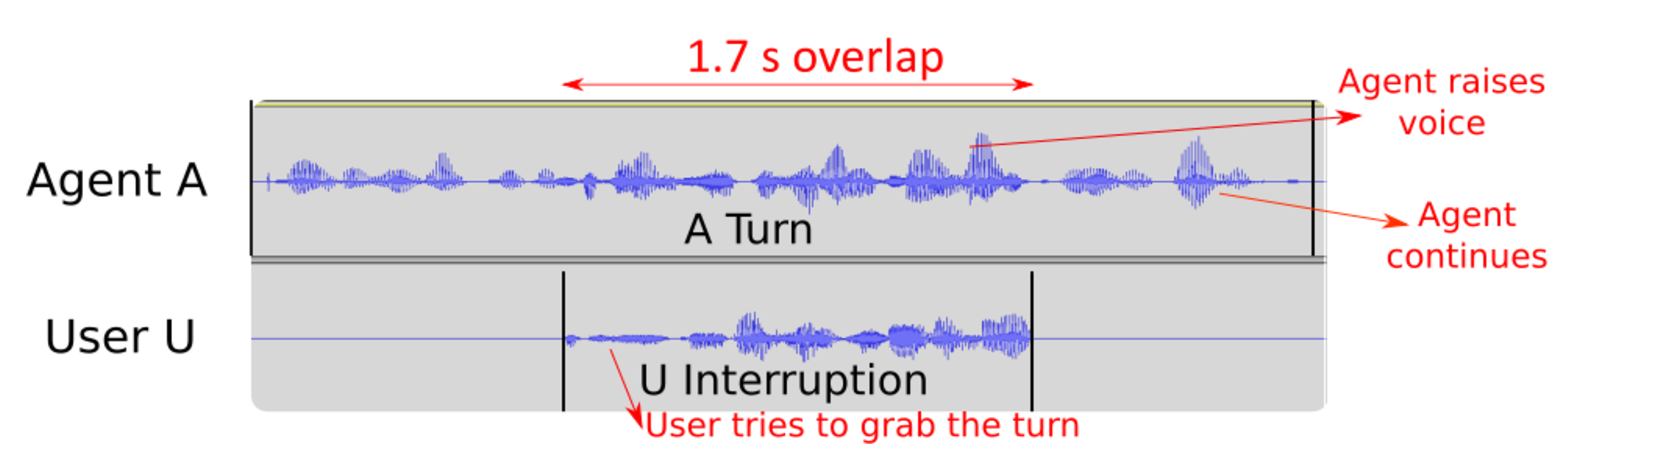
\includegraphics[width=\linewidth]{figure/volume_transcript_1_1_refait.eps}
  \caption{Illustration of the first interaction. The user attempts to grab the turn, and the agent raises its voice to prevent the user from interrupting and subsequently continues its turns after the user stops.}
  \label{sc_1}
\end{figure}

\begin{figure}
\centering
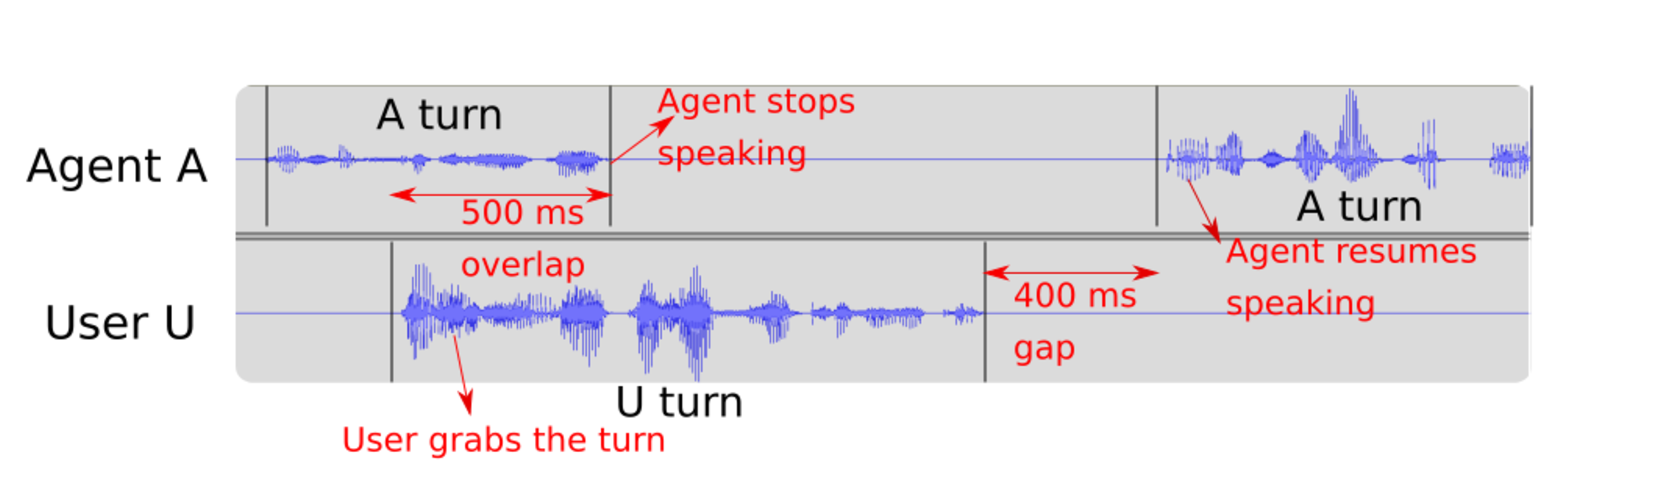
\includegraphics[width=\linewidth]{figure/volume_transcript_1_2_refait.eps}
\caption{Illustration of a scenario whereby the agent stops in response to the user barging in.}
\label{sc_2}
\end{figure}

\begin{figure}
\centering
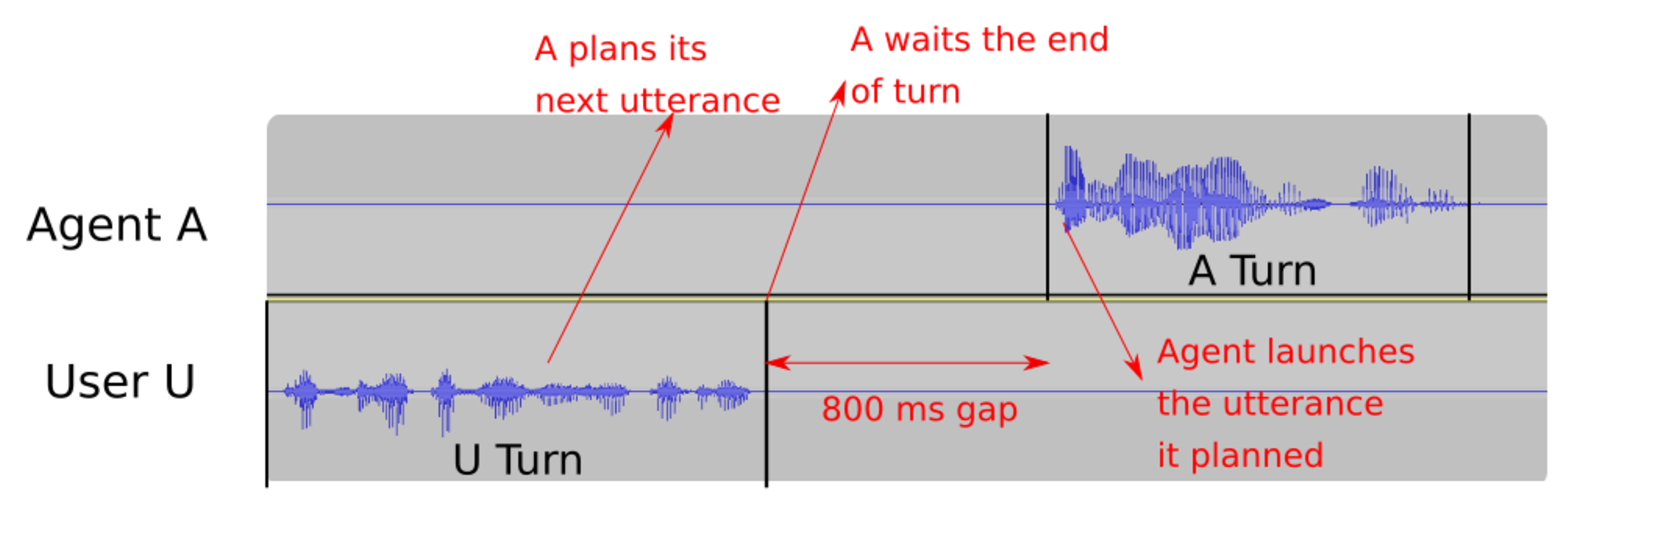
\includegraphics[width=\linewidth]{figure/volume_transcript_2_2_refait.eps}
\caption{Illustration of a scenario whereby the agent waits until the end of the turn of the user even if it has understood was the latter was saying.}
\label{sc_3}
\end{figure}

\begin{figure}
\centering
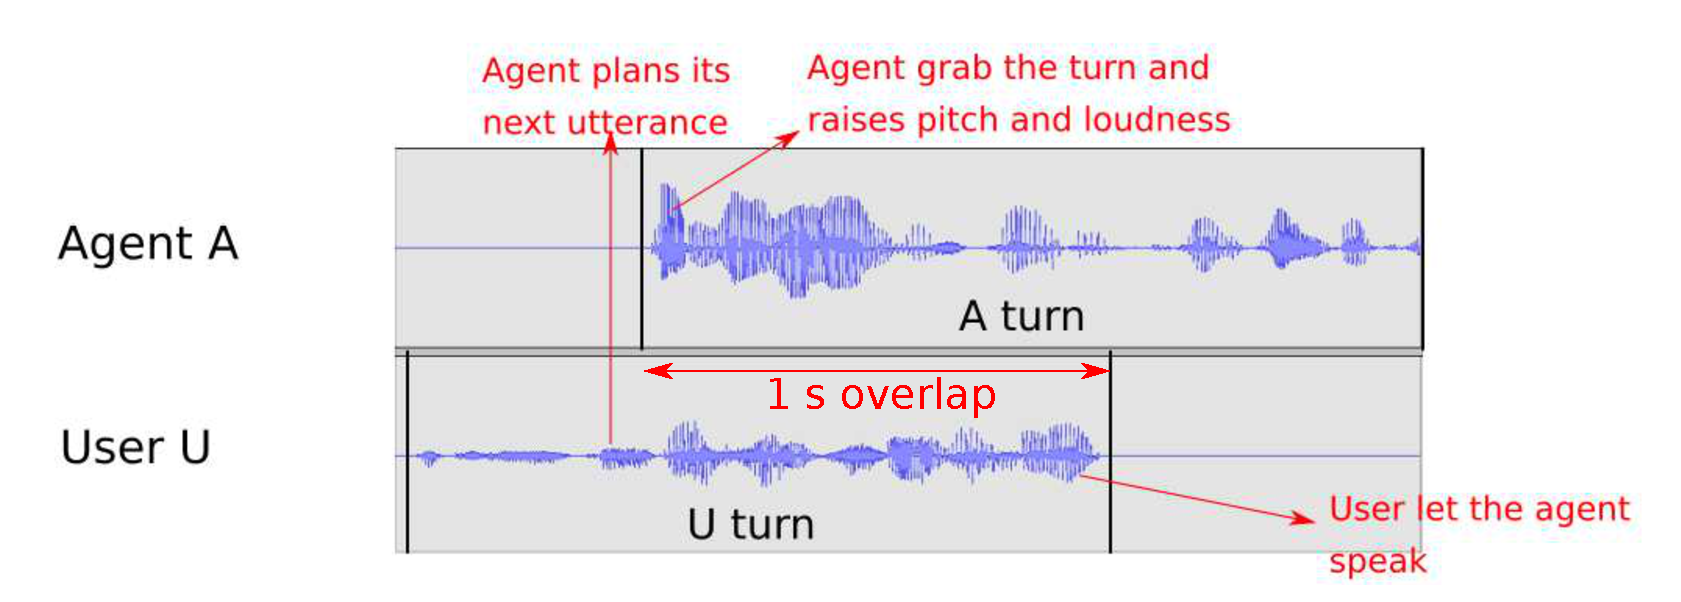
\includegraphics[width=\linewidth]{figure/volume_transcript_2_1_refait.eps}
\caption{Illustration of a scenario whereby the agent interrupts the user as soon as it has understood what the user was saying.}
\label{sc_4}
\end{figure}

Figure \ref{sc_3} illustrates the second interaction: the agent was the current listener and had a weak motivation to answer the user's question, although it had understood what the user was saying before the end of the user's turn. In this situation, the agent did not start speaking before the end of the user's question. 

Figure \ref{sc_4} shows what occurred in the same situation when the agent had a strong motivation to answer the question. 
As soon as the agent had recognized what the user was saying, the utterance generation module planned an utterance that was sent to the realizer. Nevertheless, because the loudness command of the realizer was less than the threshold, the utterance was not immediately launched in the TTS. 
Due to its weak motivation to speak, while the user was still speaking, the loudness of the agent remained lower than the 'silence' threshold. When the user had finished the turn, the accumulation value begun to increase toward a positive value. When this accumulation value reached a given (high) value, the loudness attractor increased, making the loudness parameter further increase. As soon as this parameter became higher than the value of the silence threshold, the realizer launched the utterance into the TTS.
The fact that the agent, in this situation, waited a while before starting to speak was due to how we defined the loudness control equations. In these equations, depending on the motivation value, the loudness begins to increase above a positive accumulation value: the lower the motivation, the higher the accumulation value has to be for the loudness to increase. If its motivation increases, the agent will begin to speak sooner and, as an extreme, will interrupt the user. Figure \ref{sc_4} shows that when the agent's motivation is very strong, a long turn overlap occurs. 

\section{Evaluation of real-time interactions between the user and the agent}
\label{sec:eval}

\subsection{Motivation}
\label{subsec:mot}

This evaluation aimed at answering three questions: 
(i) Is an agent controlled by our model able to smoothly coordinate its speaking turns with the user?
(ii) How does the user perceive the agent's interruptions as controlled by our model?
(iii) How do different turn-taking behaviors impact the agent's credibility, user's satisfaction and ease of interaction with the agent? Do different turn-taking behaviors influence the user's turn-taking behavior? 

Our methodology was based on existing evaluation techniques.
\cite{skantze_towards_2010} and \cite{de_vault_toward_2015} conducted two studies to evaluate  an agent's turn-taking management in the context of negotiation scenarios. In these experiments, the agents were, at least partially, controlled by a Wizard of Oz (WOz). In \cite{skantze_towards_2010}, only the user's utterances were transcribed by the WOz, the remaining being managed by the system. The user's ends of turns were identified using a voice activity detector, and the agent systematically responded to the user after detecting the end of the user's turn. In \cite{de_vault_toward_2015}, the whole process, from interpretation to generation, was managed by the Wizard of Oz, including turn-taking management. These two experiments had the advantage of answering research questions similar to ours. First, the agent's coordination ability was evaluated through a comparison of the agent's response time and overlap duration with human interactions. Second, the agent's credibility, the user's satisfaction and the ease of interaction with the agent were evaluated through questionnaires. The ability of the agent to correctly signal its intentions toward turn-taking was not directly treated. However, some behaviors of the user, such as the user's latency to take the turn after the end of the agent's turn, were analyzed. In our view, these behaviors could be related to the ability of the user to clearly identify signals displayed by the agent: the clearer the agent's signals, the shorter the user's response latencies. These evaluations seemed particularly adapted to our own objective, and thus, we based our methodology on these evaluations. Nevertheless, one major difference is that in our study, the agent's turn-taking behavior varied according to the outputs of our model. 

\subsection{Protocol}

Similarly to \cite{de_vault_toward_2015} and \cite{skantze_towards_2010}, we conducted an experiment whereby the user and the agent were engaged in a negotiation scenario. The interaction was an audio-only interaction; the agent had no graphical representation. The agent could only perceive and control two prosodic parameters: the loudness and pitch of the voice. 
The scenario staged two participants on board a sinking boat preparing to embark on a life boat. 
Each participant had different beliefs about the situation. 
One thought that they were close to the coast, and thus, the priority was to reach the coast as soon as possible. 
The other thought that they were far from the coast, the priority here being to survive in the life boat as long as possible. 
According to their beliefs, they had to make a shared decision about three items to take with them in the life boat among six items. We chose different items such that three of them were adapted to the first situation and three were adapted to the second situation.
This scenario led the user, given his own belief, to disagree with the agent's proposals, a situation favoring turn grabbing and leading to potential interruptions.   

We used our implementation presented in Section \ref{impl}. The agent had thus a complete turn-taking module that determined when the agent utterance should be launched. To avoid user utterance misinterpretations, we chose to replace the Automatic Speech Recognizer and Response Planning components by a Wizard of Oz. The WOz listened and selected utterances using an interface that allowed him to select arguments in favor of the items that the agent wanted to take and to produce counter-arguments to the user's proposals. It was necessary to avoid any influence of the Wizard of Oz's response time on the agent turn-taking behavior. To that end, the WOz was instructed to select the agent's next utterance before the end of the user's utterance. 
To make the WOz answer as fast as possible, the interface was organized into buttons, determining the different dialog acts. In order to vary the utterances pronounced by the agent, a list of utterances was associated with each button. Each time the WOz clicked the corresponding button, the system iterated on the list of utterance and selected the next utterance. The chosen utterance was then sent to the agent that determined when to launch the utterance according to the output of the turn-taking module, using the mechanism presented in Section \ref{impl}. To achieve the most natural interactions, the utterances that the agent could produce were collected from a corpus of human interactions that we collected before for the same scenario.

To assess the coordination ability of our agent, we compared our turn-taking model (M1) with an implementation of a second model (M2). 
In this second model, we used a voice activity detector to detect moments where the user was speaking. 
The second turn-taking module was implemented following the following rules: 
\begin{itemize}
\item when no speech activity is detected after 600~ms, consider that the user has finished its turn and take the turn;
\item after at least 100~ms of speech activity, consider that the user is beginning a new turn and stop speaking. 
\end{itemize} 
These rules based on a temporal threshold are often used in spoken dialog systems and agent architectures \citep{ward_root_2005}. Interestingly, they are considered as non-optimal \citep{ward_root_2005}. The two thresholds of 600~ms and 100~ms corresponded to values used in existing models (see for example \citep{ferrer_is_2002}). 

When the agent was controlled by our model M1, it was able to modulate its prosodic signals and thus inform the user about its intention by decreasing the pitch and loudness of its voice at the end of the turn as well as raising its pitch and loudness to inform the user about its intention to grab the turn.  
With model M2, the agent was unable to vary its prosodic signals and thus had no non-verbal modality to convey any information about its intention. 

To assess whether the agent turn-taking behavior influenced the user's judgment and behavior, we defined two different behaviors according to the agent's role. In the first case, the agent systematically released the turn when it detected that the user wanted to grab the turn, and it systematically waited until the end of the user's turn before taking the turn (weak motivation to take or keep the turn). In the second case, the agent insisted on keeping the turn when it detected that the user wanted to grab the turn, and it systematically attempted to grab the turn (strong motivation to take or keep the turn). To generate these two behaviors, we varied the motivation value. 
For the first behavior, the motivation was set to $m=-0.4$ when the agent was the speaker and to $m=0.4$ when the agent was the listener. In the second condition, $m=-1.0$ when the agent was the speaker, and $m=1.0$ when the agent was the listener.

We ensured that the user interacted equally with the agent having  weak and strong motivation to take and keep the turn, respectively. To that end, we divided the interaction into two parts. In the first part, the user interacted with an agent having a weak motivation to take or keep the turn, and in the second part, the user interacted with an agent with a strong motivation.
% the user interacted with an agent having a strong motivation to take and keep the turn. 
We maintained this order for all the interactions because beginning the interaction with an agent systematically attempting to grab or keep the turn would risk making the user refuse to continue to engage in the interaction with the agent. 

Finally, we collected the user's judgments about the agent using a questionnaire (Table \ref{Answers}) with questions about the ease of interaction with the agent (question Q9 in Table \ref{Answers}), the user's satisfaction (Q8, Q10) and agent credibility (Q11). The corresponding questions were adapted from \cite{skantze_towards_2010}, \cite{bevacqua_effects_2014} and \cite{de_vault_toward_2015}. Moreover, to assess the clarity of the agent's signals, we added questions about the intentionality of the agent's interruptions, that is, whether the agent's interruptions were due to an agent mistakenly perceiving the user's ends of turns or where made by the agent on purpose (Q3 and Q4). Finally, we added questions about the ability of the agent to smoothly coordinate its turns with the user (Q1, Q2, Q5, Q6, and  Q7). For each item, the participant had to declare its level of agreement, between strongly disagree and strongly agree on a continuous scale between 0 and 10. 

The different conditions of the experiments were as follows.
In condition 1, the user interacted with an agent controlled by model M1.
In condition 2, the user interacted with an agent controlled by model M2.
Condition 1 presented two variants, depending of the value of the motivation parameter: ``condition 1 strong'' and ``condition 1 weak''. 
Each participant interacted with the agent twice, each time under a different condition.
The order of the conditions (``condition 1" and ``condition 2") was counterbalanced between participants. For each condition, the interaction lasted 2 min 30 s. The questionnaire was presented to the participant at the end of each condition. We also recorded the audio of the user and the audio of the agent on separate channels. We finally logged several events occuring during the experiment: the moments when the agent's utterances were launched by the TTS system and moments when the WOz selected an utterance by clicking on the corresponding button. 


\subsection{Results}

31 volunteers (30 males and 1 female) participated in the experiment. They were all native French speakers and were students, engineers or researchers. We describe in the following sections the analysis that we conducted to answer the three questions presented in Section \ref{subsec:mot}.

\subsubsection{Is the agent able to smoothly coordinate its speaking turns with the user?}

First, we analyzed the duration of the user-to-agent transitions (Figure \ref{box_ua}). This assessed the ability of the agent to rapidly identify and react to the user's end of turn. For this analysis, we manually annotated the turns of the participants. This allowed us to identify moments when the agent or the user began and ended their turns. From these manual annotations, we computed transition durations as the difference in seconds between the beginning of the next turn and the end of the previous turn. We called overlaps, transitions with a negative transition duration. We also combined beginning and end-of-turn data to the moments when the WOz had selected an utterance. This allowed us to distinguish transitions where the WOz selected an utterance before the user's end of turn and transitions where the WOz selected an utterance after the user's end of turn. We discarded the latter transitions for further analysis, as their durations were solely due to the WOz reaction time and not to the performance of the turn-taking module. Moreover, in this analysis we did not consider overlaps because they were due to mistakes in the perception of the end of the user's turn by the WOz; we analyzed them separately.

We found that under ``condition 1 weak", the agent took the turn more rapidly (average: 840~ms) compared to the second condition (1.19~s), the difference being significant (p$<$0.05). However, we also observed a high number of mistakes in the detection of the user's ends of turns under all conditions, with almost 50 \% of transitions having at least slight overlaps.  
Finally, we analyzed the responses to questions Q1, Q2, Q5, Q6 and Q7 (Table \ref{Answers}), referring to the user's subjective perception of the agent's ability to coordinate its speaking turns. We did not find significant differences between the conditions. Generally speaking, participants found that the agent was able to coordinate its turn with them, with low scores for questions Q1, Q2 and Q6. 
Nevertheless, the answers to question Q7 showed that the users noticed long moments of silence whereby they believed that the agent did not want to speak. 
 
\begin{figure}
\centering
\includegraphics[width=\linewidth]{figure/boxTransitionsUA.pdf}
\caption{Durations of silence during User-to-Agent transitions (gaps in seconds).}
\label{box_ua}
\end{figure}
  
\begin{table}
\centering
\resizebox{\linewidth}{!}{\begin{tabular}{|p{3cm}|p{2cm}|p{2cm}|p{2cm}|}
\hline
Questions & Median \linebreak conds. 1 & Median \linebreak cond. 2 & p-value \\
\hline
Q1: My interlocutor \linebreak did not perceive the moment were I talked & 2.25 & 1.75 & 0.95\\
\hline
Q2: My interlocutor took the turn randomly& 2.5 & 2.625 & 0.6 \\
\hline
Q3: My interlocutor interrupted involuntarily& 6 & 4 & 0.019* \\
\hline
Q4: My interlocutor interrupted me on purpose& 6 & 6.5 & 0.91 \\
\hline
Q5: My interlocutor paid attention not to interrupt me & 4.5 & 7.5 & 0.006**\\
\hline
Q6: My interlocutor was slow to respond to me & 3 & 2 & 0.77\\
\hline
Q7: My interlocutor refused sometimes to speak to me & 6.125 & 5.75 & 0.16\\
\hline
Q8: My interlocutor annoyed me by the way he took the turn & 4.5 & 3.25 & 0.54\\
\hline
Q9: I was at ease interacting with my interlocutor & 5.25 & 6.25 & 0.55\\
\hline
Q10: I liked speaking with my interlocutor & 6.625 & 7 & 0.52\\
\hline
Q11: The behavior of my interlocutor was close to the behavior of a human speaker & 5.625 & 6.5 & 0.97\\
\hline
\end{tabular}}
\caption{Mean agreements of the participants for conditions 1 and condition 2 (translated from French).}
\label{Answers}
\end{table}

\subsubsection{How does the user perceive the agent's interruptions?}

By analyzing the answers to questions Q3 and Q4, we found that the users classified the agent's interruptions as intentional or unintentional under condition 1 (scores higher than 5 for the two conditions) even if the users only slightly agreed with assertions Q3 and Q4. Logically, participants perceived that the agent paid greater attention not to interrupting them under condition 2 compared to condition 1. 
We completed this analysis with measurements of the user's behavior during interruptions. We found that the pitch of the user was significantly greater than the mean pitch during conflictual moments for ``condition 1 strong''. This means that under this condition, the user seemed to react in a specific manner to the interruptions made on purpose by the agent. Very interestingly, this reaction was not observed under the other conditions wherein the agent involuntarily overlapped with  the user's speech.


\begin{figure}
\centering
\includegraphics[width=\linewidth]{figure/boxTransitionsAU.pdf}
\caption{Durations of silence during Agent to User transitions (gaps in seconds).}
\label{box_au}
\end{figure}

\subsubsection{How do different turn-taking behaviors impact the agent's credibility, user's satisfaction and ease of interacting with the agent?}

Generally speaking, the participants liked speaking with the agent (question Q10), but the results of the question related to the credibility of the agent were more mitigated (Q11), with a median of 6.5 for the assertion ``The behavior of my interlocutor was close to the behavior of a human speaker" under the second condition and 5.6 under the first condition. The users also answered that they were at ease during the interaction (Q9) even if they did not strongly agree with the assertion and did not seem annoyed by the agent's turn-taking behavior (Q8). 
We finally assessed the impact of the conditions on the user's ability to coordinate himself with the agent by measuring the duration of the agent-to-user transitions. We found that under condition 1, the user took the turn more rapidly (average: 1.11~s) compared to condition 2 (average: 1.39~s), the difference being significant (p$<$0.05). 


\subsection{Discussion}

The results show that our model allows the agent to smoothly coordinate its turns with users. Indeed, the agent took the turn faster under ``condition 1 weak" compared to ``condition 2". Under all conditions, we observed a great proportion of unintentional overlaps (50 \% of user-agent transitions) due to mistakes in the perception of the user's end of turn. This high rate of false detections was partly due to the voice activity detector used to detect when the user was speaking: logs revealed numerous moments whereby no voice was detected but where the user was actually speaking. 
Answers to questions Q1, Q2, Q6 and Q7 show that the users did not clearly perceive the improved coordination capability provided by our model. The fact that the participants did not seem to be disturbed by the relatively long duration of the user-to-agent transitions supports the idea that they did not expect optimal turn transitions from the agent.

Moreover, when investigating how users perceived the agent's interruptions, we observed that the users almost equally considered  that the agent interrupted them unintentionally or on purpose when the agent raised its volume and pitch to inform the user about its intention to grab the turn (our model) or when the pitch and volume were not modulated. However, we found that users increased their pitch when interrupted by the agent only under ``condition 1 strong". This led us to believe that users distinguished, at least implicitly, the intentional or unintentional nature of the interruptions and varied their behavior accordingly. We can conclude that solely raising pitch and loudness did not seem to sufficiently inform of the agent's intention to grab the turn. The lack of distinction between intentional interruptions and those due to mistakes in the detection of the user's end of turn could be due to difficulties encountered by the participants in perceiving the agent's pitch and loudness variations. These difficulties could come from the quality of the voice synthesizer that we used, participants often having reported a poor quality of the voice. 
At the end of the experiment, we collected the oral impressions of the participants concerning the interaction. The participants were divided when asked about their perception of the agent's interruptions. Six participants explicitly mentioned that they perceived the agent's interruptions as non-voluntary; on the other hand, thirteen participants perceived at least some interruptions as voluntary. 

 Interestingly, we found that users took the turn faster with our model. Two hypotheses can explain this difference. 

First, users could have perceived the decrease in the pitch and loudness of the agent's voice, thereby helping them to identify the agent's willingness to end its turn. 
Second, differences in agent-user transition durations could be the result of an alignment effect: the fact that the agent took the turn faster led the user to take the turn faster. This hypothesis is plausible, as such alignment has been observed in human conversations \citep{levitan_entrainment_2015}.  

Finally, the analysis of the answers to the questionnaire shows that the variation in the agent's behavior does not seem to have a significant impact on a user's judgment about the interaction. 
However, oral impressions collected after the interaction are not as categorical.   
For instance, the perception of the interruptions seems to be conducive to more positive impressions. Four participants judged interruptions as coherent and credible given the dialog context, and five participants associated these interruptions with the fact that the agent did not agree or attempted to impose its own ideas, which is consistent. 
Finally, among the thirteen participants, five participants judged these interruptions as human-like. On the other hand, one of the participants reported a feeling of rage linked to the incessant interruptions of the agent, and two participants reported that they were annoyed by these interruptions. We could explain the differences in these impressions by the fact that the agent interrupted the user regardless of the dialog context. This could result in moments whereby the agent's interruptions seemed inappropriate, whereas others were particularly relevant to the context. Therefore, interruptions could give an impression of smoothness and immersion in the dialog under the condition that they are consistent with the context of the dialog, which is what the variation in the motivation parameter of our model attempts to account for.

\section{Conclusion}

\subsection{Contributions of this article}

We presented three different contributions in this article. First, we developed a theoretical model for the coordination of speaking turns between a user and an agent. Our assumption is that the coordination of turns is partly an emergent property that originates from the sensorimotor coupling between the participants. 
The agents controlled by our theoretical model are adaptive: they are able to ensure coordination in different types of environment and in interactions with partners that have more or less inertia in producing their signals or more or less rapidly perceive  the behavior of their partner. Even if we presented only two types of adaptations,  namely, to the absence or presence of signals and to how the user produces his signals, the simulations show the capability of an emergent model to reproduce the situations linked to the coordination of turns observed in human conversations.

This adaptability is essential, as there exists a variety of ways users coordinate their turns with the agent. The adaptation is based on the idea that the participants continuously modify  their verbal and non-verbal productions to ensure effective coordination. This highlights the fact that not only must the agent be able to reliably perceive  the user's intentions but also the user has to reliably perceive  the agent's behavior in different environmental settings. One way to guarantee that the user will still reliably perceive the agent's behavior is for the agent to adapt its behavior to clarify its intentions to the user, a capacity that we observed in our simulations without needing to modify the equations controlling the signal productions. This view of user-agent adaptation is new in the context turn-taking, as past approaches relied on offline machine learning techniques or online reinforcement learning to reliably perceive the behavior of the user without considering how the user perceives the agent's behavior. 

However, this principle of adaptation also requires the ability for the user to adapt his signal production to clarify his behavior and intentions. Whether the user could adapt his behavior to both the agent and environment is currently an open research issue and requires further analyses of user-agent interactions. 
Some clues lead us to believe that a type of adaptation of the user to the agent is done, as we observed a variability in the silence durations after the end of the agent's turn and before the user's beginning of turn regardless of whether the user interacted with the agent controlled by our model or with an agent controlled by a model based on temporal thresholds. Nevertheless, we do not know the exact reason for this variability; it could be due to the prosodic signals produced by the agent at the end of its turn or linked to a temporal alignment of the user to how the agent takes the turn, a phenomenon observed in human conversations. 

As a second contribution, we proposed an agent architecture, named BeAware, for the implementation of both continuous and discrete control models of behavior. 
Indeed, very few embodied conversational agents can combine these two types of model. 
Our solution is an extension of the ASAP architecture \cite{kopp_architecture_2014}, enriched with principles borrowed to Ymir \citep{thorisson_mind_1999}. 
The solution complies with the SAIBA standard, and thus, our model can be integrated with existing modules that manage other aspects of multimodal user-agent interactions such as expressive verbal production, emotions and interpersonal attitudes. Such abilities require one to implement realizers for managing concurrently, among others, the prosody, the gestures, head movements, and the gaze direction of the agent.

Finally, we analyzed how the agent's turn-taking strategy may impact the user's experience and the effectiveness of the coordination.
We measured factors related to the credibility of the agent, the user's satisfaction and the ease of interaction.  
Undoubtedly, the quality of the coordination is multifactorial and requires one to finely perceive and modulate a rich set of verbal and non-verbal signals. It also requires effective incremental speech recognition and generation. None of the existing components supporting these processes have achieved the desired quality to support natural interactions. Our experiment showed that users do not always interpret the agent's turn-taking as voluntary but rather as implementation artifacts and thus experienced difficulties in coordinating with the agent. 
However, our experimental setup had certain limitations. 
First, the coordination was only based on the modulation of the prosody. Introducing other perceptual channels should enrich the information available for the coordination, thus making it more effective.
Second, we focused on the most critical situations, namely, long overlaps of speaking turns. Under these conditions, the agent should have been able to modify its verbal contents when barging in during interactions with the users (e.g., word recycling and use of fillers). This inconsistency may explain the manner in which participants perceived the agent's behavior. 
Finally, we manually set the parameters of the control equations. Optimizing these parameters should result in a better coordination. 

\subsection{Future work}

As mentioned in Section \ref{backgd}, verbal content is a main source of information for listeners to detect ends of turns \cite{de_ruiter_projecting_2006} and should  help participants to coordinate their speaking turns considerably. Nevertheless, the way in which one could implement the interpretation mechanism in an embodied conversational agents remains unclear. The first reason is because the process used by human participants to coordinate turns based on verbal information is still being debated \citep{heldner_pauses_2010,magyari_prediction_2012,riest_anticipation_2015}. Te second reason is because the method hypothesized by a majority of authors implies reliably  perceiving word by word the utterances of the user and being able to perceive and reason about the syntax of the utterance in real time \citep{sacks_simplest_1974}, capacities that current natural language understanding components barely support \cite{de_vault_incremental_2011}.

Moreover, in all interaction scenarios presented in this article, the agent's motivation with respect to turn-taking was set manually and remained constant throughout the interaction. To achieve a more realistic turn-taking process, this motivation should vary in real time according to the context of the interaction and to the agent's state.
While past computational models linked interpersonal attitudes \citep{ravenet_conversational_2015} or importance of the verbal contribution \citep{selfridge_bidding_2009} with turn-taking behaviors, no model has explored the links between the agent's emotional state and its turn-taking behavior. We plan to address this question by adding a module that computes the motivation variable according to the agent's emotions.

Finally, in human conversations, when participants are motivated to be and remain listeners, they produce backchannels to inform the current speaker that they are still listening to what he is saying and may even encourage him to continue speaking. 
We could exploit our motivation variable to trigger and drive some behaviors related to grounding such as backchannels. 
For the speaker, the detection of backchannels could impact its perceptual decision-making process, as a user producing backchannels likely does not take the turn immediately.
We also plan to explore in greater detail the mechanism of alignment linked to the coordination of turns, as highlighted by \citep{benus_pragmatic_2011}.
We hypothesize that our model could account for the temporal alignment observed in human conversations.  

\bibliographystyle{spmpsci}

\bibliography{jmui}

\end{document}
